\section{Overview}

\draftchange{This chapter presents the results obtained from laboratory power consumption testing, preliminary field trials at Háskóli Íslands, LoRa range evaluation, long-term deployment in Keldur, and soil moisture calibration. The results are analyzed in relation to the system requirements defined in Chapter 3, particularly long-term low-power operation, communication performance of the installed sensor nodes, mesh network operation, and calibration accuracy. The Keldur deployment demonstrated the system under real outdoor conditions, while the calibration tests characterized the response of the soil moisture sensor over the tested 0--40\% range using a calibration soil sample.}

\section{Power Consumption
Results}

\subsection{Packet Sending Time
Calculation}

The in situ sensor node operates under a strict duty cycle constraint,
remaining active for a maximum of 5 minutes per hour while spending the
remaining 55 minutes in deep sleep. The transition from deep sleep to
full operation, including sensor activation via MOSFET, data
acquisition, and shutdown, takes approximately 3.1 seconds.

LoRa packet airtime is determined by the sum of preamble and payload
durations:

\begin{equation}
T_{packet} = T_{preamble} + T_{payload}
\label{eq:packet-airtime}
\end{equation}

With spreading factor \(SF = 10\), bandwidth
\(BW = 125\text{ }\text{kHz}\), and preamble length
\(N_{preamble} = 8\), the symbol time is:

\begin{equation}
T_{sym} = \frac{2^{SF}}{BW} = \frac{2^{10}}{125000} = 0.008192\text{ }\text{s}
\label{eq:symbol-time}
\end{equation}

The preamble duration is therefore:

\begin{equation}
T_{preamble} = (N_{preamble} + 4.25) \cdot T_{sym} \approx 0.1\text{ }\text{s}
\label{eq:preamble-duration}
\end{equation}

The payload duration depends on the payload size \(PL\) \draftchange{and} is given by:

\begin{equation}
T_{payload} = N_{payload} \cdot T_{sym}
\label{eq:payload-duration}
\end{equation}

For the selected configuration (CRC enabled, explicit header, low data
rate optimization, coding rate 4/5), this simplifies to:

\begin{equation}
N_{payload} = 8 + 5 \cdot \left\lceil \frac{8PL + 4}{32} \right\rceil
\label{eq:payload-symbols}
\end{equation}

Thus, total packet airtime becomes:

\begin{equation}
T_{packet} = \left( 20.25 + 5 \cdot \left\lceil \frac{8PL + 4}{32} \right\rceil \right) \cdot 0.008192
\label{eq:total-packet-airtime}
\end{equation}

For a 96-byte payload, the airtime is approximately 1.19 seconds per
transmission.

Assuming six sensor data types (e.g., temperature, humidity, soil
temperature, battery level, and timestamp) are transmitted eight times
per hour, the total transmission time is:

\begin{equation}
(1.19\text{ }\text{s} \times 8) \times 6 \approx 57\text{ }\text{s}
\label{eq:hourly-transmission-time}
\end{equation}

This is approximated to 1 minute of transmission time per hour. Then we
can assume that the rest is spent receiving LoRa packets and operating
in standby mode, which is approximately 237 seconds.

\clearpage
\subsection{Operating Modes}

\begin{longtable}[]{@{}
  >{\raggedright\arraybackslash}p{(\columnwidth - 6\tabcolsep) * \real{0.2457}}
  >{\raggedright\arraybackslash}p{(\columnwidth - 6\tabcolsep) * \real{0.2026}}
  >{\raggedright\arraybackslash}p{(\columnwidth - 6\tabcolsep) * \real{0.1634}}
  >{\raggedright\arraybackslash}p{(\columnwidth - 6\tabcolsep) * \real{0.3884}}@{}}
\caption{Operating states, measured current consumption, and duration per hour.}
\label{tab:operating-modes}\\
\toprule\noalign{}
\begin{minipage}[b]{\linewidth}\raggedright
\textbf{Operating State}
\end{minipage} & \begin{minipage}[b]{\linewidth}\raggedright
\textbf{Measured Current (mA)}
\end{minipage} & \begin{minipage}[b]{\linewidth}\raggedright
\textbf{Duration per Hour}
\end{minipage} & \begin{minipage}[b]{\linewidth}\raggedright
\textbf{Notes}
\end{minipage} \\
\midrule\noalign{}
\endfirsthead
\endhead
\bottomrule\noalign{}
\endlastfoot
Deep Sleep & 0.3 mA & 55 minutes & All modules off, MCU in deep sleep \\
Awake (Sensors ON / LoRa OFF) & 9.5 mA & 3 s & Sensor initialization and
data acquisition \\
LoRa RX/TX & 119.5 mA & 60 s & Transmission and reception of LoRa
packets \\
Half Sleep & 12.2 mA & 237 s & Sensors off, MCU in low-power mode, LoRa
in standby \\
\end{longtable}

\draftchange{During the laboratory test described in Section~\ref{sec:power-tests}, each operating state was maintained for 10 seconds to allow the current reading to stabilize. The measurement routine was observed over three complete loops to verify repeatability. The durations per hour shown in Table~\ref{tab:operating-modes} represent the operating-cycle durations used for the weighted average current calculation; they were not the duration of the laboratory measurement itself. Therefore, the average current consumption of approximately 3.08 mA is a calculated hourly cycle average based on the measured current in each operating state and its corresponding operating duration, rather than a direct average-current measurement taken over a continuous one-hour test.}

The average current consumption is calculated as:

\begin{equation}
I_{avg} = \frac{\sum I_{n}t_{n}}{T}
\label{eq:average-current}
\end{equation}

where \(I_{n}\) \draftchange{is} the current in each state, \(t_{n}\) \draftchange{is} the duration of
each state, and \(T = 3600\text{ }\text{s}\) \draftchange{is} the total time per hour.

Substituting the measured values:

\begin{equation}
\begin{aligned}
I_{avg} &=
\frac{(0.3 \times 3300) + (9.5 \times 3) + (119.5 \times 60)
+ (12.2 \times 237)}{3600} \\
&= \frac{990 + 28.5 + 7170 + 2891.4}{3600} \\
&\approx 3.08\,\text{mA}
\end{aligned}
\label{eq:average-current-substitution}
\end{equation}

Thus, the average current consumption of the sensor node under
worst-case conditions is approximately \textbf{3.08 mA}.

Given a total battery capacity of 10,500 mAh (three 3,500 mAh cells in
parallel), the estimated operational lifetime is:

\begin{equation}
\frac{10500}{3.08} \approx 3409\text{~hours} \approx 142\text{~days~}( \sim 4.7\text{~months})
\label{eq:three-cell-lifetime}
\end{equation}

This estimate assumes ideal battery performance. In practice,
environmental factors---particularly low temperatures in Iceland---will
reduce effective battery capacity and shorten the operational lifetime.

For comparison, a single 3,500 mAh cell would yield an estimated
lifetime of approximately:

\begin{equation}
\frac{3500}{3.08} \approx 1136\text{~hours} \approx 47\text{~days}
\label{eq:single-cell-lifetime}
\end{equation}

This highlights the importance of parallel battery configuration for
extended deployment.

\draftchange{Overall, the estimated operating lifetime is considered sufficient for the intended application.} Turf roofs are periodically inspected and maintained,
allowing battery replacement to be integrated into routine maintenance
cycles. This ensures continuous operation of the sensor nodes while
supporting long-term monitoring of soil conditions and turf roof
integrity.

\section{Initial Field
Deployment}

\draftchange{An initial field test was conducted on the University of Iceland (Háskóli Íslands) campus, with sensor nodes positioned approximately 50--100 m from the base station.} The primary objective of
this deployment was not to evaluate the final performance of the system,
but rather to validate the functionality of the preliminary hardware,
firmware, and communication system under real outdoor conditions. Since
turf roofs are present at several buildings on campus, including the
turf-covered bicycle shed, these locations provided an accessible
environment for testing while allowing rapid troubleshooting and
hardware modifications during development.

Four prototype sensor nodes (HW\_1, HW\_3, HW\_5, and HW\_7) were
deployed to collect air temperature, relative humidity, soil
temperature, and soil moisture data. Measurements were transmitted
through the LoRa network to the base station and uploaded to the cloud
for analysis. \draftchange{Measurements from the prototype sensor nodes were cross-checked against observations from the Reykjavík Hljómskálagarður automatic weather station (Station 1469), operated by Veðurstofa Íslands~\cite{imo_observations}.}

\subsection{Air Temperature and Relative
Humidity}

Figure~\ref{fig:results-1} compares the measured air temperature from the prototype
sensor nodes with the \draftchange{Reykjavík Hljómskálagarður weather station (Station 1469)}, while Figure~\ref{fig:results-2} presents
the corresponding relative humidity measurements.

\begin{figure}[htbp]
\centering
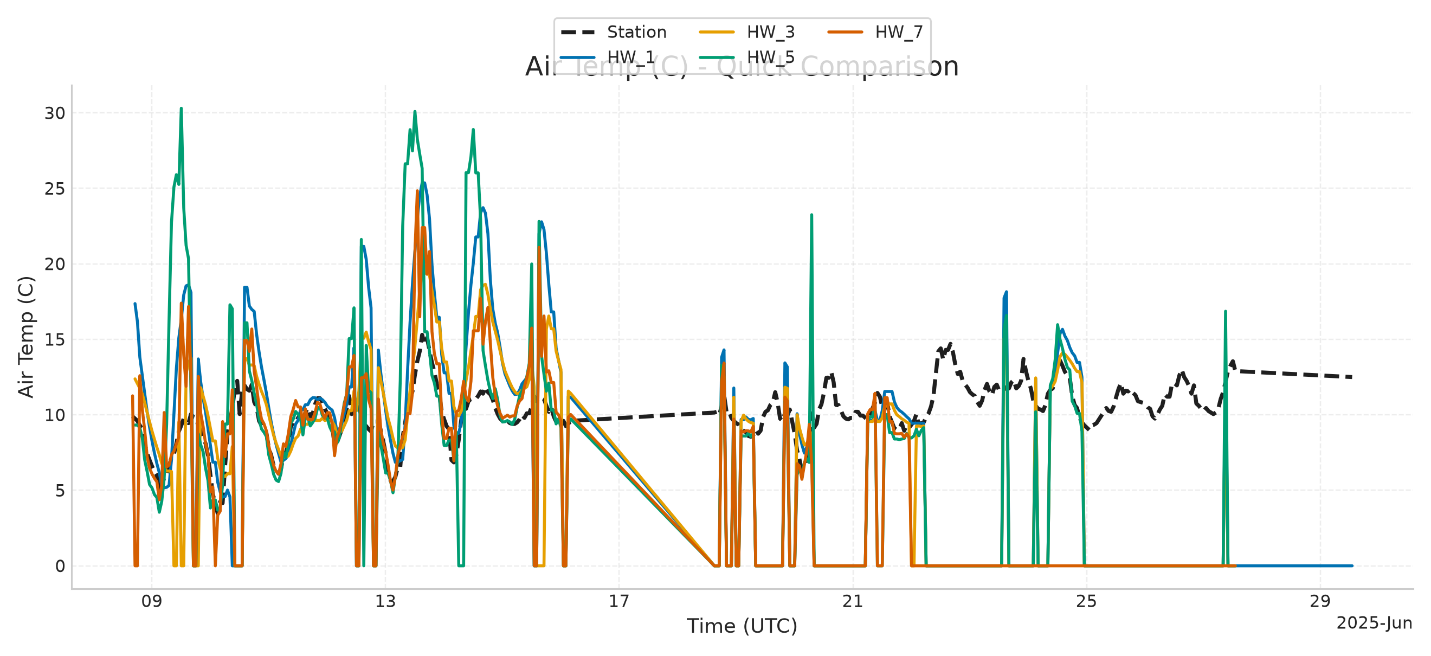
\includegraphics[width=\textwidth,height=2.97917in,keepaspectratio]{figs/results-image1.png}
\caption{Air temperature measurements during the preliminary field deployment.}
\label{fig:results-1}
\end{figure}

\begin{figure}[htbp]
\centering
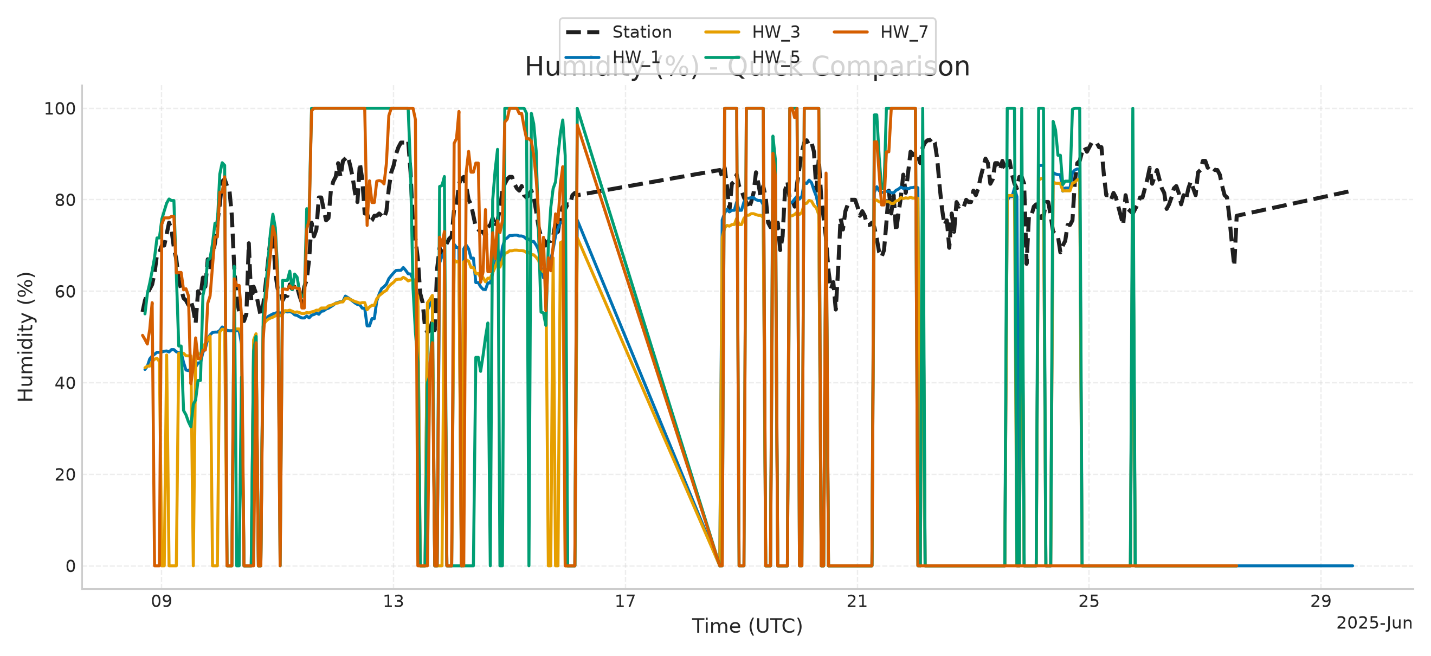
\includegraphics[width=\textwidth,height=2.97917in,keepaspectratio]{figs/results-image2.png}
\caption{Relative humidity measurements during the preliminary field deployment.}
\label{fig:results-2}
\end{figure}

The prototype nodes successfully collected environmental measurements
throughout the deployment period and generally followed the overall
trends observed by the weather station. However, numerous interruptions,
missing samples, and unstable readings were observed. These
inconsistencies were expected because the firmware and hardware were
still under active development, with frequent updates and adjustments
being performed throughout the testing period.

\draftchange{The comparison with the weather station was intended as a contextual cross-check of general environmental trends. It was not a direct calibration or an absolute accuracy validation, because the sensor nodes and the weather station were located at different sites.}

One of the major issues identified during this deployment was poor LoRa
communication performance. During testing, the sensor nodes were
initially equipped with commercially available antennas that were later
found to be designed primarily for Wi-Fi frequencies rather than the
\textbf{433 MHz LoRa frequency} used by the system. As a result, signal
quality was significantly degraded, leading to frequent packet loss,
communication interruptions, and incomplete datasets. This issue was
identified during the preliminary deployment and later resolved by
replacing the antennas with properly tuned 433 MHz LoRa antennas before
the final deployment.

\subsection{Soil Temperature and Soil
Moisture}

Figure~\ref{fig:results-3} presents the measured soil temperature, while Figure~\ref{fig:results-4}
shows the corresponding soil moisture measurements collected during the
preliminary deployment.

\begin{figure}[htbp]
\centering
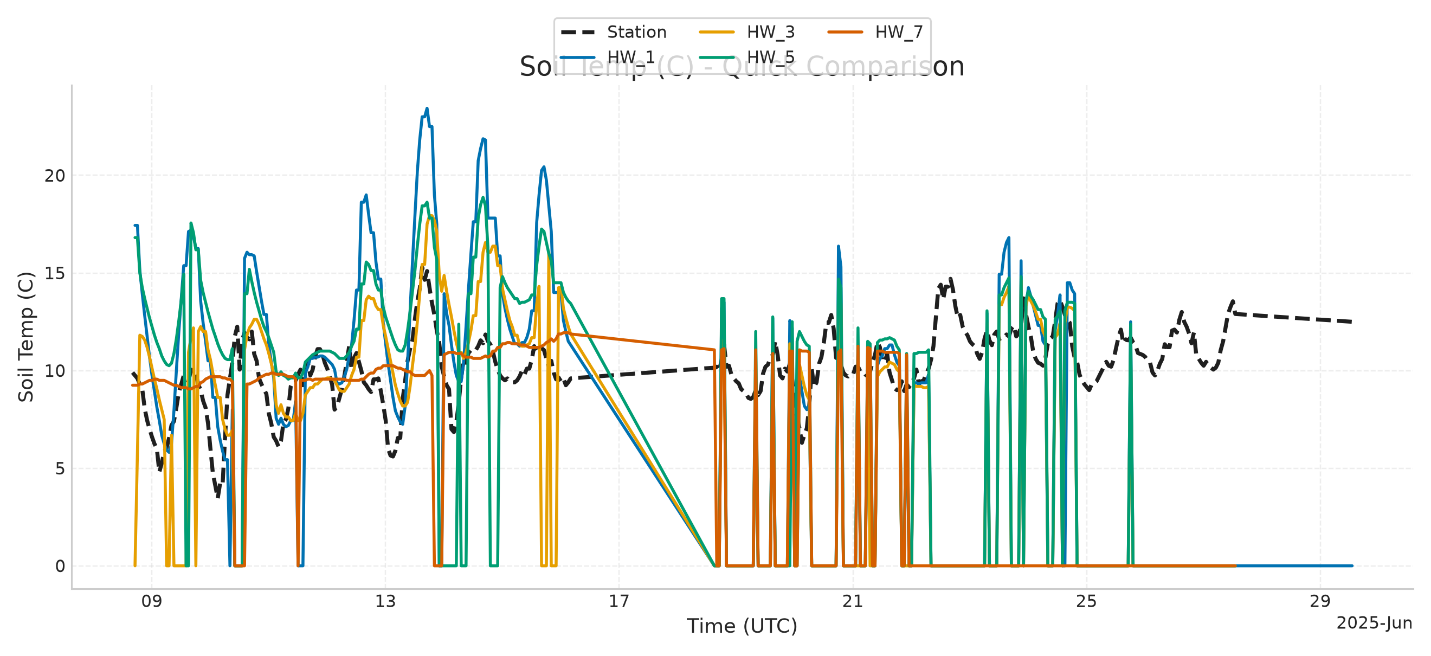
\includegraphics[width=\textwidth,height=2.97917in,keepaspectratio]{figs/results-image3.png}
\caption{Soil temperature measurements during the preliminary field deployment.}
\label{fig:results-3}
\end{figure}

\begin{figure}[htbp]
\centering
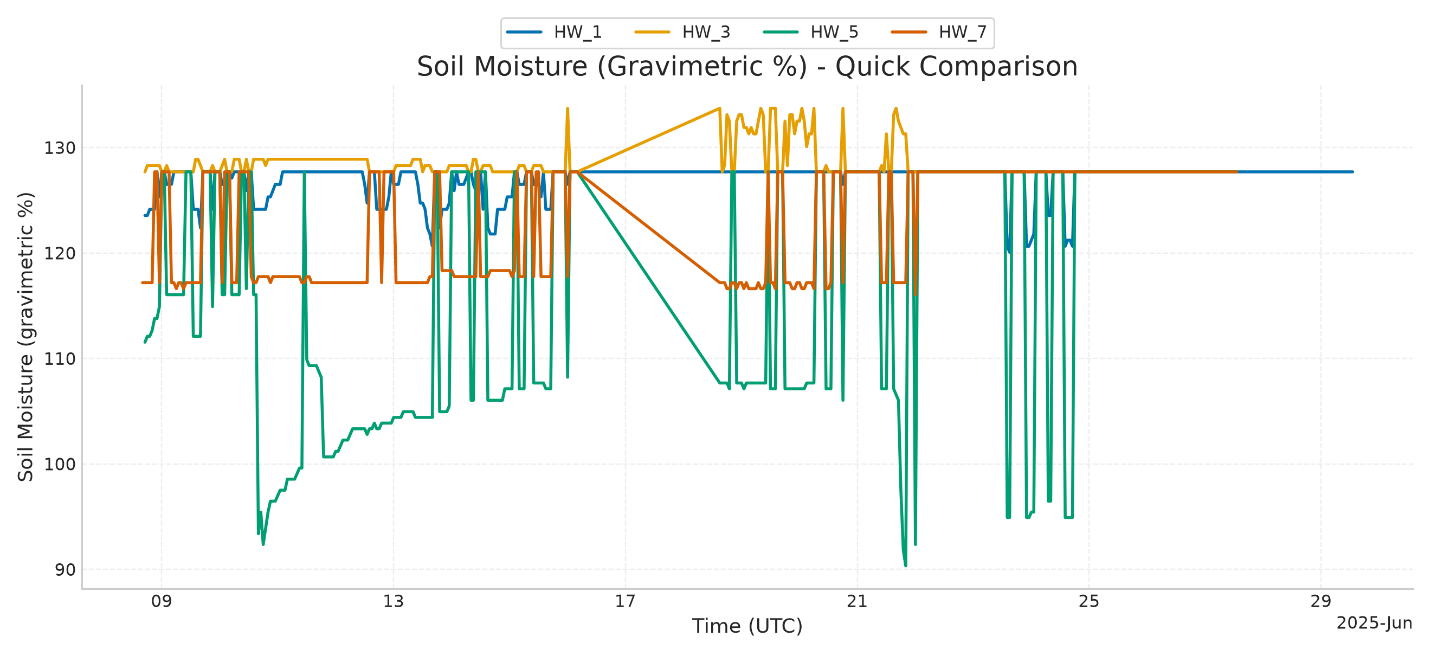
\includegraphics[width=\textwidth,height=2.97917in,keepaspectratio]{figs/results-image4.png}
\caption{Soil moisture measurements during the preliminary field deployment.}
\label{fig:results-4}
\end{figure}

The prototype sensor nodes successfully measured subsurface temperature
and soil moisture while installed beneath the turf roofs. Similar to the
later deployments, soil temperature exhibited considerably smaller
fluctuations than ambient air temperature due to the thermal buffering
properties of the surrounding soil.

The soil moisture measurements, however, showed considerable variability
and several unrealistic values exceeding the expected physical range. At
this stage of development, the moisture sensors had not yet undergone
final calibration, and firmware updates affecting sensor scaling were
still being tested. Combined with the communication issues caused by the
incorrect antennas, the resulting datasets contained numerous missing
samples and erroneous measurements. Nevertheless, the deployment
successfully demonstrated that the sensing hardware, analog measurement
circuitry, and cloud logging system operated correctly under outdoor
conditions.

\subsection{Summary of Preliminary
Testing}

The preliminary field deployment successfully fulfilled its intended
purpose as an engineering validation phase. Although the collected
environmental data were not suitable for scientific analysis due to
communication interruptions and ongoing hardware development, the
testing identified several important issues that were subsequently
corrected. Most notably, replacing the incorrectly matched antennas with
antennas specifically designed for the 433 MHz LoRa frequency
significantly improved communication reliability and packet delivery in
later deployments. Additional improvements included refinements to the
firmware, sensor calibration procedures, enclosure design, and overall
system stability.

\draftchange{Local SD card backup was implemented and tested. During the earlier testing, the measurements stored on the SD card were used to fill missing or blank values in the collected dataset where wireless transmissions had been missed. This showed that the local storage could be used to recover data that had not reached the base station during communication interruptions.}

The knowledge gained from this preliminary deployment formed the basis
for the final hardware revision used in the subsequent long-term field
deployment, where substantially improved communication reliability and
data quality were achieved.

\clearpage
\section{LoRa Range Testing Results (Vellir --
Hafnarfjörður)}\label{sec:lora_range_testing}

\subsection{Test Configurations}

The following configuration parameters were used during the LoRa field
range testing:

\begin{lstlisting}[
    caption={LoRa configuration parameters used during field range testing.},
    label={lst:lora-test-config},
    basicstyle=\normalsize\ttfamily,
    breaklines=true,
    captionpos=b,
    escapeinside={(*@}{@*)}
]
#define FREQUENCY       433E6   // 433 MHz
#define TX_POWER        17      // dBm
#define BANDWIDTH       125E3   // 125 kHz
#define SYNC_WORD       0x12
#define SPREAD_FACTOR   10
#define CODING_RATE     5
#define PREAMBLE        8
\end{lstlisting}

During the initial field test, communication performance was limited due
to the use of antennas designed for Wi-Fi rather than LoRa. These
antennas were not tuned for the 433 MHz operating frequency, resulting
in significantly reduced range. After replacing them with antennas
designed specifically for LoRa frequencies, a substantial improvement in
communication performance was observed.

Field testing was conducted in a semi-urban environment around Vellir in
Hafnarfjörður. Using the configuration described above, reliable
communication was achieved within an approximate radius of 3 km. Signal
quality improved when the transmitting node was positioned at elevated
locations, highlighting the importance of antenna placement.

In areas with dense infrastructure, such as residential zones with
multiple buildings obstructing the line of sight, signal degradation and
occasional packet loss were observed. This confirms that LoRa
performance is strongly influenced by environmental obstructions and
benefits from relatively clear propagation paths.

\begin{figure}[htbp]
\centering
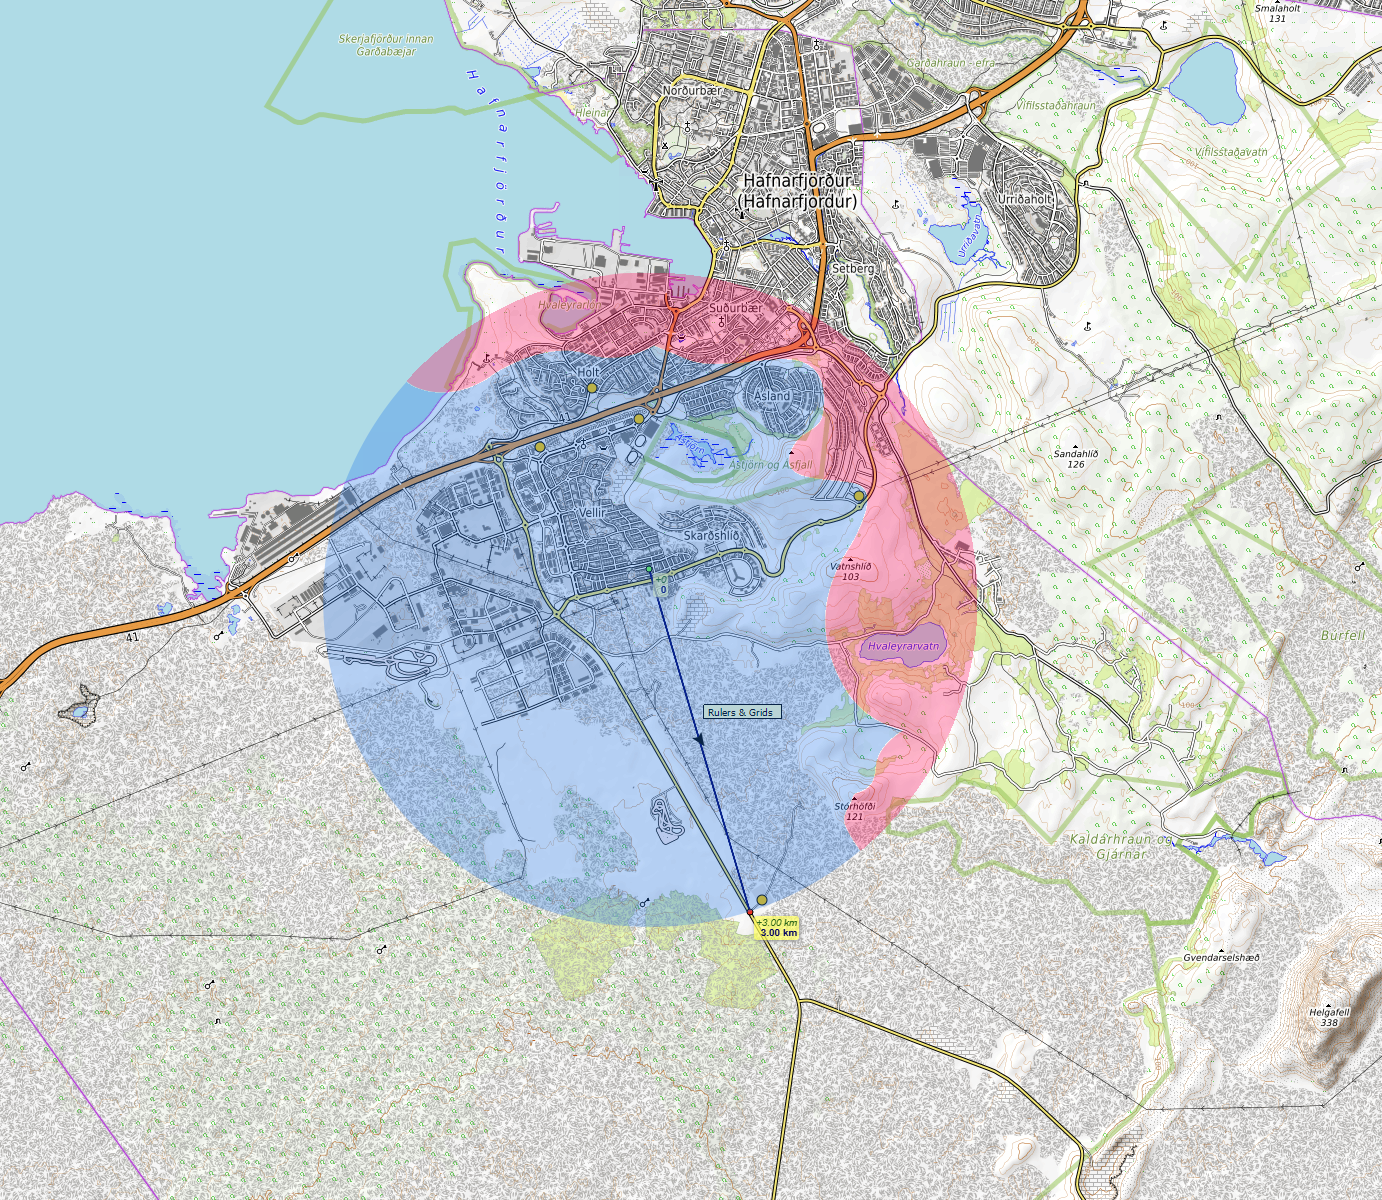
\includegraphics[width=\textwidth,height=5.64583in,keepaspectratio]{figs/results-image5.png}
\caption{Estimated LoRa signal coverage map for the Vellir--Hafnarfjörður field test. Blue regions indicate reliable communication coverage at approximately 3 km, while red regions indicate weak or absent signal strength due to terrain and structural obstructions.}
\label{fig:results-5}
\end{figure}

\draftchange{The estimated signal coverage map is shown in Figure~\ref{fig:results-5}.} Regions marked in red represent areas where no signal was
detected, primarily due to terrain obstructions such as hills and dense
built environments.

Signal strength measurements were recorded at multiple locations within
the testing area. The average RSSI values are summarized in the RSSI table.

\begin{table}[htbp]
\centering
\caption{Average RSSI values recorded at each test location during the LoRa range evaluation.}
\label{tab:rssi-summary}
\begin{tabular}{p{0.55\textwidth} p{0.25\textwidth}}
\toprule
\textbf{Location} & \textbf{Average RSSI} \\
\midrule
Ásvallalaug & -113 dBm \\
Holt & -103 dBm \\
Fish Drying Area & -112 dBm \\
Vatnslíð & -103 dBm \\
Netto & -112 dBm \\
\bottomrule
\end{tabular}
\end{table}

\subsection{Discussion of Results}

\draftchange{The results demonstrate reliable single-hop LoRa communication within an approximate 3 km radius. The recorded RSSI values, ranging from -103 dBm to -113 dBm, provide a useful indication of the communication performance achieved with the selected radio configuration and antennas.}

\draftchange{The Vellir range test evaluated direct, single-hop communication only; it did not evaluate the mesh relay process. A separate informal relay test was conducted during firmware development (Section~\ref{sec:informal-multihop}). Sensor nodes were spaced apart, and the researcher observed debug output showing ledger data being forwarded between nodes and eventually reaching the base station. Because this test was not logged and its topology, node count, spacing, and firmware revision were not retained, it provides qualitative evidence that the relay mechanism operated but does not provide measured multi-hop range, packet-delivery ratio, hop count, or latency. A controlled, logged multi-hop test is still needed to quantify those performance measures. Actual performance in turf-roof installations will also depend on antenna placement, burial depth, terrain, and surrounding structures.}

\section{Intermediate Field
Deployment}

Following the preliminary field testing, an intermediate field
deployment was conducted to evaluate the performance of the revised
hardware after replacing the original antennas with antennas
specifically designed for the \textbf{433 MHz LoRa operating frequency}.
The deployment was again carried out at several turf roof locations
around the \textbf{University of Iceland (Háskóli Íslands)} campus,
allowing rapid access to the sensor nodes for hardware modifications and
firmware updates while operating under real outdoor conditions.

The primary objective of this deployment was to verify the improvements
in LoRa communication reliability, evaluate the stability of the
environmental sensors, and identify any remaining hardware or software
issues before proceeding to the final long-term deployment. Four sensor
nodes (HW\_1, HW\_3, HW\_5, and HW\_7) continuously monitored air
temperature, relative humidity, soil temperature, and soil moisture,
while measurements from the \draftchange{Reykjavík Hljómskálagarður weather station (Station 1469) were used as a contextual cross-check.}

\subsection{Air Temperature and Relative
Humidity}

\draftchange{Figure~\ref{fig:results-6} compares the measured air temperature from the four prototype sensor nodes with the Reykjavík Hljómskálagarður weather station (Station 1469), while Figure~\ref{fig:results-7} presents the corresponding relative humidity measurements. As in the preliminary deployment, this comparison is a contextual cross-check of general trends rather than a calibration or absolute accuracy validation, because the instruments were located at different sites.}

\begin{figure}[htbp]
\centering
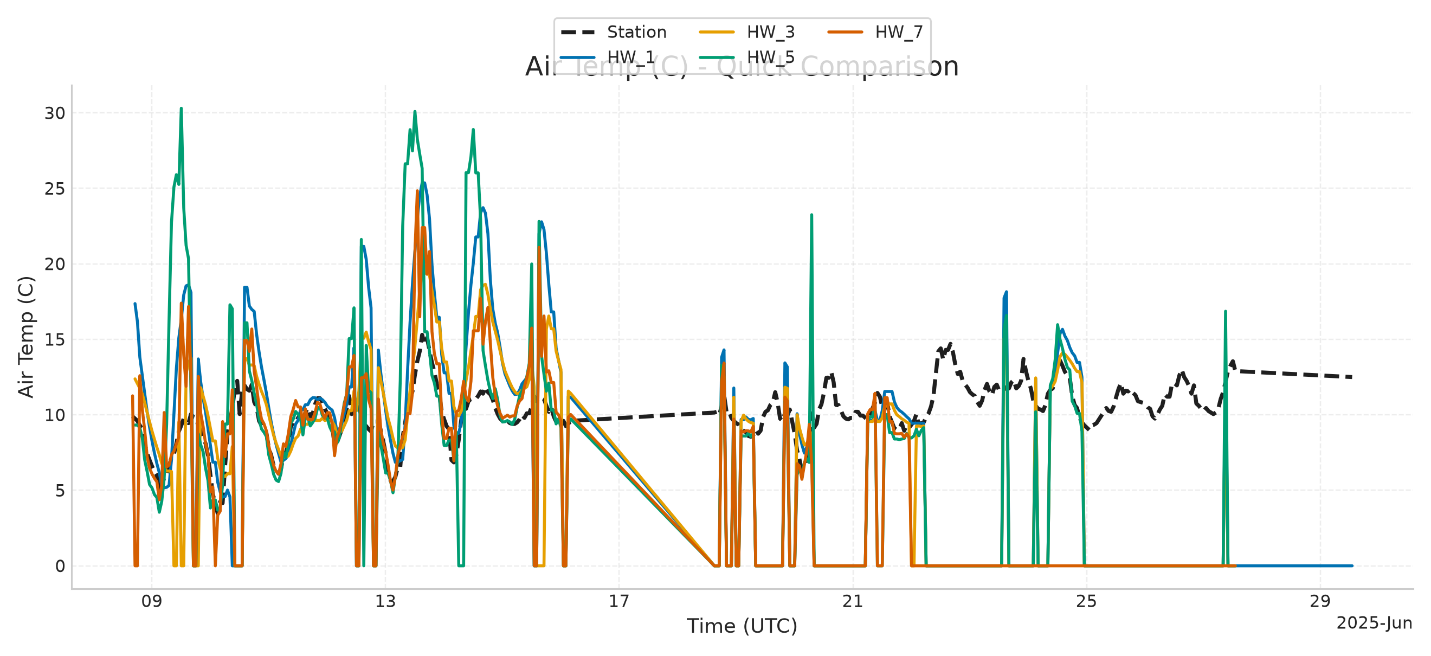
\includegraphics[width=\textwidth,height=2.97917in,keepaspectratio]{figs/results-image1.png}
\caption{Air temperature measurements during the intermediate field deployment.}
\label{fig:results-6}
\end{figure}

Compared with the preliminary deployment described in Section 4.3,
replacing the antennas with properly matched \textbf{433 MHz LoRa
antennas} resulted in a noticeable improvement in communication
reliability. Longer periods of uninterrupted environmental data were
successfully transmitted to the base station, reducing the amount of
missing data caused by packet loss.

The measured air temperatures generally followed the same trends as the
\draftchange{Reykjavík Hljómskálagarður weather station}, demonstrating that the revised communication
hardware allowed more consistent data collection. Relative humidity
measurements also became more stable; however, occasional readings of
\textbf{0\%} and \textbf{100\%} were still observed. These values were
attributed primarily to ongoing firmware development and sensor
initialization issues rather than communication failures. Since the
system remained under active development, firmware updates and hardware
adjustments continued throughout the testing period.

\begin{figure}[htbp]
\centering
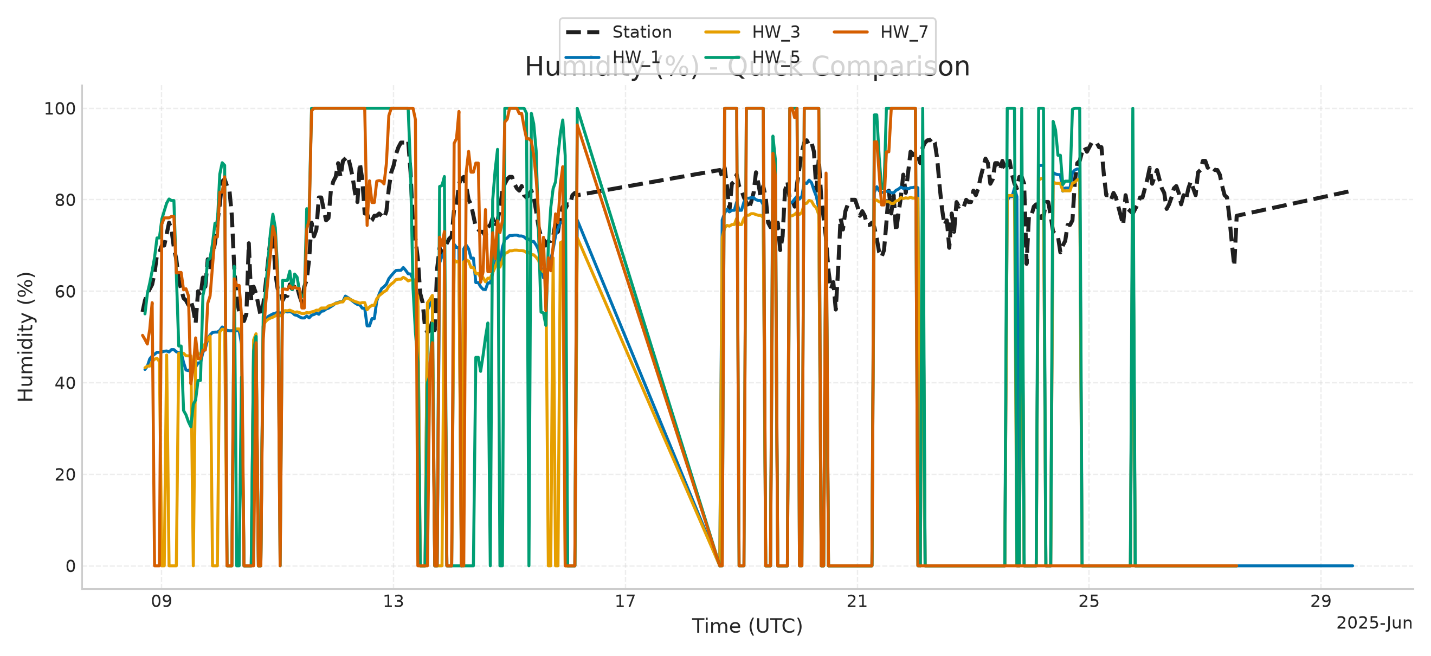
\includegraphics[width=\textwidth,height=2.97917in,keepaspectratio]{figs/results-image2.png}
\caption{Relative humidity measurements during the intermediate field deployment.}
\label{fig:results-7}
\end{figure}

\subsection{Soil Temperature and Soil
Moisture}

Figure~\ref{fig:results-10} presents the measured soil temperature from the deployed
sensor nodes, while Figure~\ref{fig:results-11} illustrates the corresponding soil
moisture measurements.

\begin{figure}[htbp]
\centering
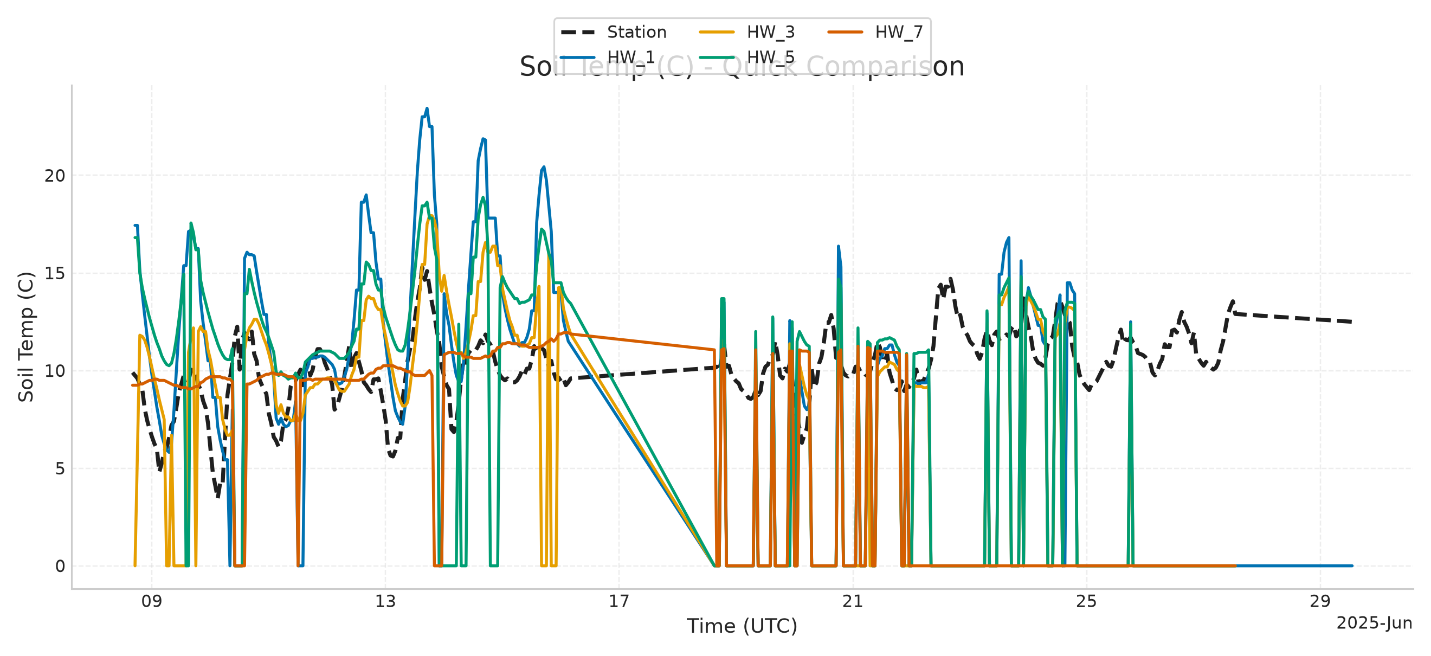
\includegraphics[width=\textwidth,height=2.97917in,keepaspectratio]{figs/results-image3.png}
\caption{Soil temperature measurements during the intermediate field deployment.}
\label{fig:results-10}
\end{figure}

Soil temperature measurements became more continuous than those obtained
during the preliminary deployment, reflecting the improved communication
performance achieved after replacing the antennas. The measured soil
temperatures remained more stable than ambient air temperatures,
demonstrating the thermal buffering effect of the surrounding soil.

\begin{figure}[htbp]
\centering
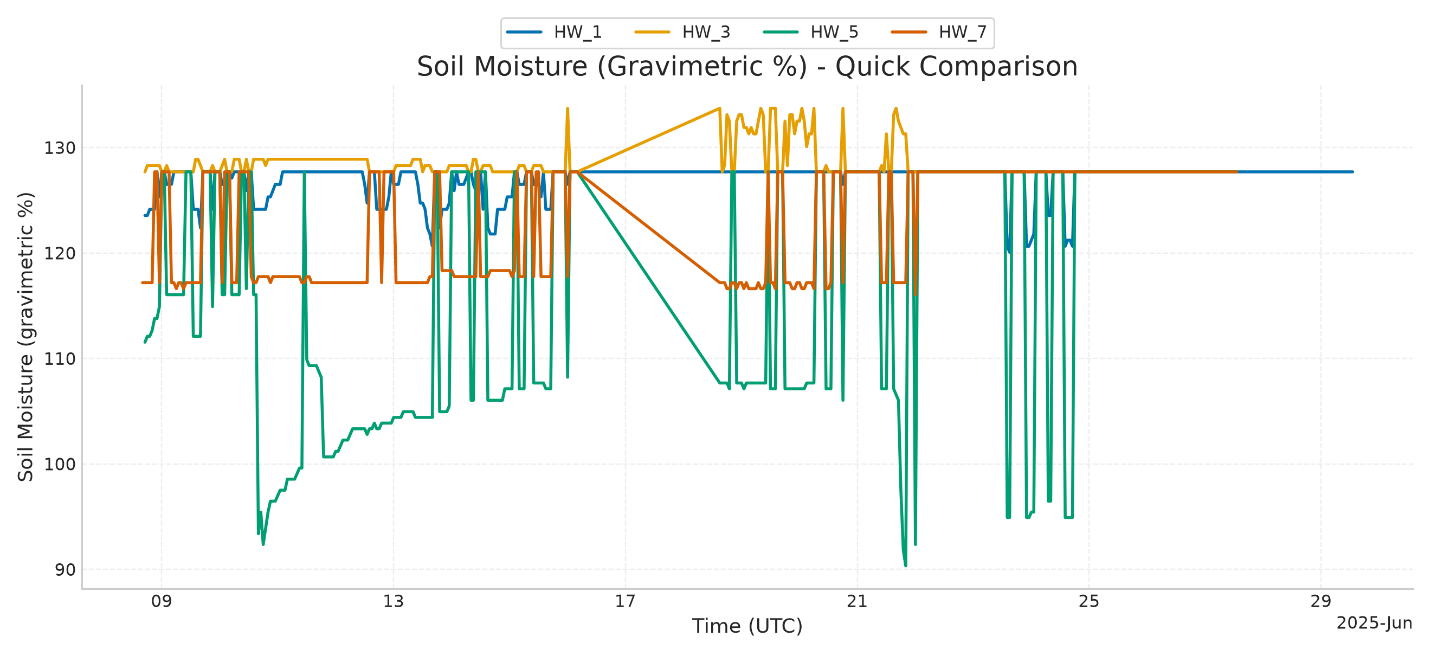
\includegraphics[width=\textwidth,height=2.97917in,keepaspectratio]{figs/results-image4.png}
\caption{Soil moisture measurements during the intermediate field deployment.}
\label{fig:results-11}
\end{figure}

The soil moisture measurements continued to exhibit considerable
variability because calibration procedures were still being refined.
Several nodes produced unrealistic values outside the expected
measurement range, indicating that further calibration and firmware
improvements were required before long-term deployment. Although these
measurements were not yet suitable for quantitative environmental
analysis, they confirmed that the sensing hardware, analog measurement
circuitry, and data logging system were operating correctly under
outdoor conditions.

\subsection{Summary}

The intermediate field deployment confirmed that replacing the original
antennas with antennas specifically designed for the \textbf{433 MHz
LoRa frequency} substantially improved wireless communication
reliability. Compared with the preliminary deployment, significantly
longer periods of continuous environmental data were successfully
collected, demonstrating that the antenna mismatch had been a major
contributor to the communication problems previously observed.

Although several issues related to firmware stability and sensor
calibration remained, the deployment successfully validated the revised
communication hardware and identified the final improvements required
before the long-term deployment. The experience gained during this stage
led to further refinements in the firmware, sensor calibration
procedures, and enclosure design, resulting in the final hardware
configuration used for the subsequent deployment at the Keldur turf
house site.

\section{Keldur Deployment}

To evaluate the performance of the proposed LoRa mesh wireless sensor
network under actual operating conditions, a field deployment was
conducted at the Keldur turf house site beginning on \textbf{17 October
2025}. Four sensor nodes (IDs 1, 3, 5, and 7) were installed at
different locations and depths beneath the turf roof. The installation
locations and sensor depths are shown in \draftchange{Figure~\ref{fig:results-deployment-map}}. Sensor Nodes
1 and 3 were designed with the air temperature and humidity sensors
enclosed inside the waterproof housing, while Sensor Nodes 5 and 7 had
these sensors mounted externally above the enclosure. This design
variation was intentionally implemented to compare the measurement
accuracy of both configurations under real environmental conditions.

\draftchange{Weather data used for comparison were obtained from the Sámsstaðir automatic weather station, operated by the Icelandic Meteorological Office (Veðurstofa Íslands), through the Icelandic Meteorological Office observation database~\cite{imo_observations}. It is commonly identified as \textit{samst}, station 6222, and has been active since 2000. It is the closest station listed on vedur.is to the Keldur test site, at a distance of 9.75 km. Its coordinates are latitude 63.735370636° and longitude -20.1090698242°.}

\clearpage
\begin{figure}[p]
    \centering
    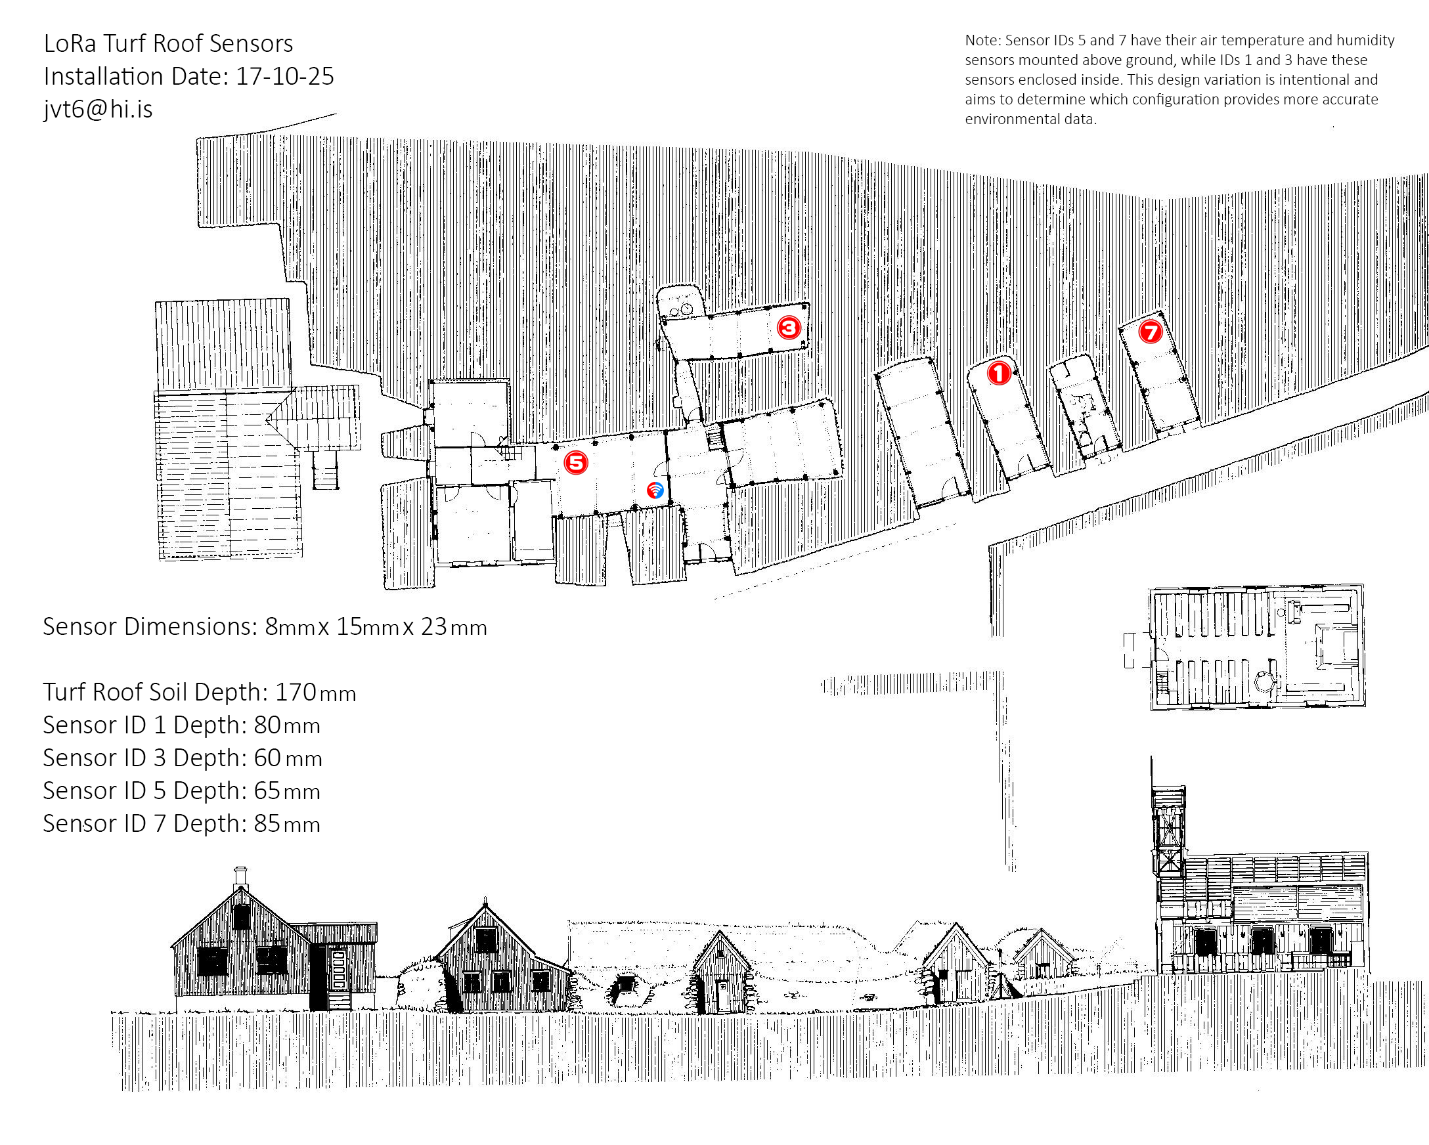
\includegraphics[
        angle=90,
        width=\textwidth,
        height=0.88\textheight,
        keepaspectratio
    ]{figs/results-image6.png}
    \caption{Deployment map showing the locations and installation depths of the four sensor nodes at the Keldur turf roof site.}
    \label{fig:results-deployment-map}
\end{figure}
\clearpage

\subsection{Air Temperature
Performance}

\draftchange{Figure~\ref{fig:results-12} compares the measured air temperature from all deployed sensor nodes with data obtained from the Sámsstaðir station (samst, 6222).}

\begin{figure}[htbp]
\centering
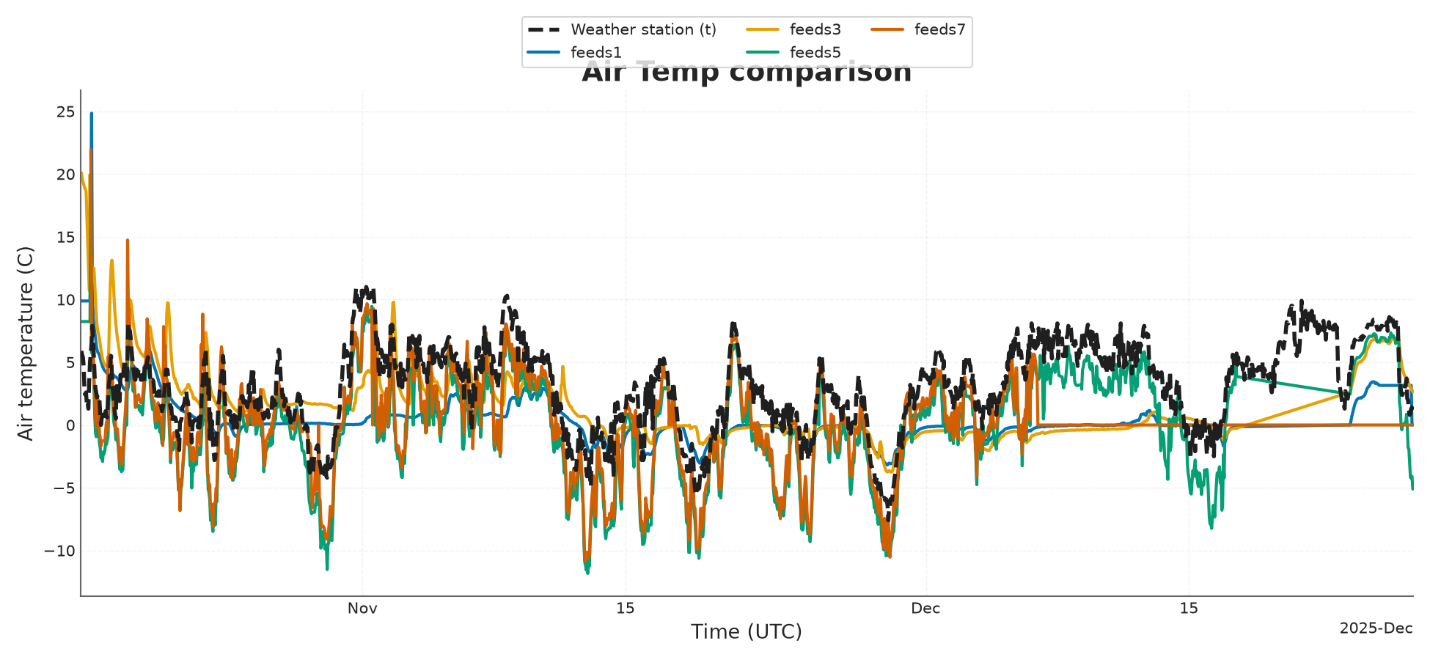
\includegraphics[width=\textwidth,height=3in,keepaspectratio]{figs/results-image7.png}
\caption{\draftchange{Comparison of air temperature measurements from the deployed sensor nodes and the Sámsstaðir station (samst, 6222).}}
\label{fig:results-12}
\end{figure}

\draftchange{The air temperature measurements from Sensor Nodes 5 and 7, which had externally mounted atmospheric sensors, generally followed the broader temperature variations observed at the Sámsstaðir weather station. Their measurements showed clearer daily fluctuations compared with Sensor Nodes 1 and 3, whose atmospheric sensors were installed inside the waterproof enclosure.}

\draftchange{The enclosed sensors produced smoother temperature curves with reduced daily variation. This suggests that placing the sensor inside the enclosure can affect how quickly it responds to changes in the surrounding air. The enclosure and its internal environment may contribute to this effect, although their individual influence was not measured separately.}

\draftchange{The average absolute temperature difference between the deployed sensors and station 6222 ranged from approximately \textbf{3.06 °C to 3.27 °C}. These values should be interpreted as differences between two measurement locations rather than direct sensor accuracy measurements. The Sámsstaðir station is approximately 9.75 km from the Keldur site, and its exposure and surrounding conditions differ from those of the deployed sensors.}

\draftchange{Overall, the observations suggest that external placement is preferable when the objective is to monitor changes in ambient air temperature. However, a co-located reference measurement would be required to evaluate the absolute accuracy of the deployed sensors.}

\subsection{Relative Humidity
Performance}\label{sec:keldur-humidity}

\draftchange{Figure~\ref{fig:results-13} presents the relative humidity measurements obtained from all deployed nodes together with reference data from the Sámsstaðir station (samst, 6222).}

\begin{figure}[htbp]
\centering
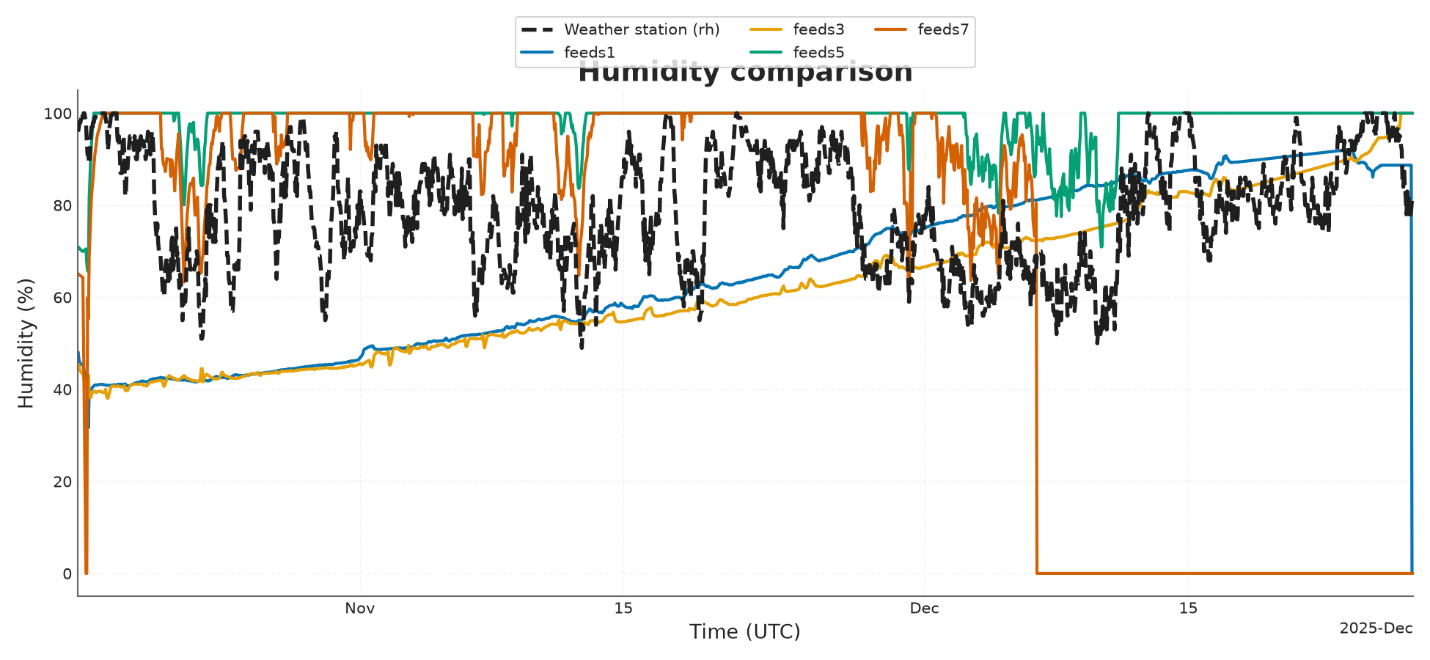
\includegraphics[width=\textwidth,height=3in,keepaspectratio]{figs/results-image8.png}
\caption{\draftchange{Comparison of relative humidity measurements from the deployed sensor nodes and the Sámsstaðir station (samst, 6222).}}
\label{fig:results-13}
\end{figure}

\draftchange{The relative humidity measurements from Sensor Nodes 5 and 7, which used externally mounted atmospheric sensors, showed broad variations that were generally comparable with the observations from the Sámsstaðir weather station. However, the comparison should be treated as qualitative because the weather station is located approximately 9.75 km from the deployment site and does not measure the exact same local conditions.}

\draftchange{Some deployed sensors produced readings that were not suitable for interpreting actual humidity variations. In particular, Sensor Node 3 recorded relative humidity values close to 100\% for an extended period toward the end of its reporting record. These readings cannot be treated as reliable evidence of the actual surrounding humidity.}

\draftchange{The available data do not establish why these readings occurred. The cause may be related to sensor exposure, moisture, the sensor environment, or another hardware or measurement issue, but the devices were not retrieved for inspection. Therefore, no specific cause should be assigned.}

\draftchange{Although the externally mounted sensors generally showed a more responsive pattern, the deployment was not a controlled experiment of sensor placement. Differences between locations and environmental exposure may also have influenced the results. Further testing would be needed to establish the effect of enclosure placement on humidity measurements.}

\subsection{Soil Temperature
Performance}

\draftchange{Figure~\ref{fig:results-14} illustrates the soil temperature measurements collected by the four buried sensor nodes together with ground-level temperature data from the Sámsstaðir station (samst, 6222).}

\begin{figure}[htbp]
\centering
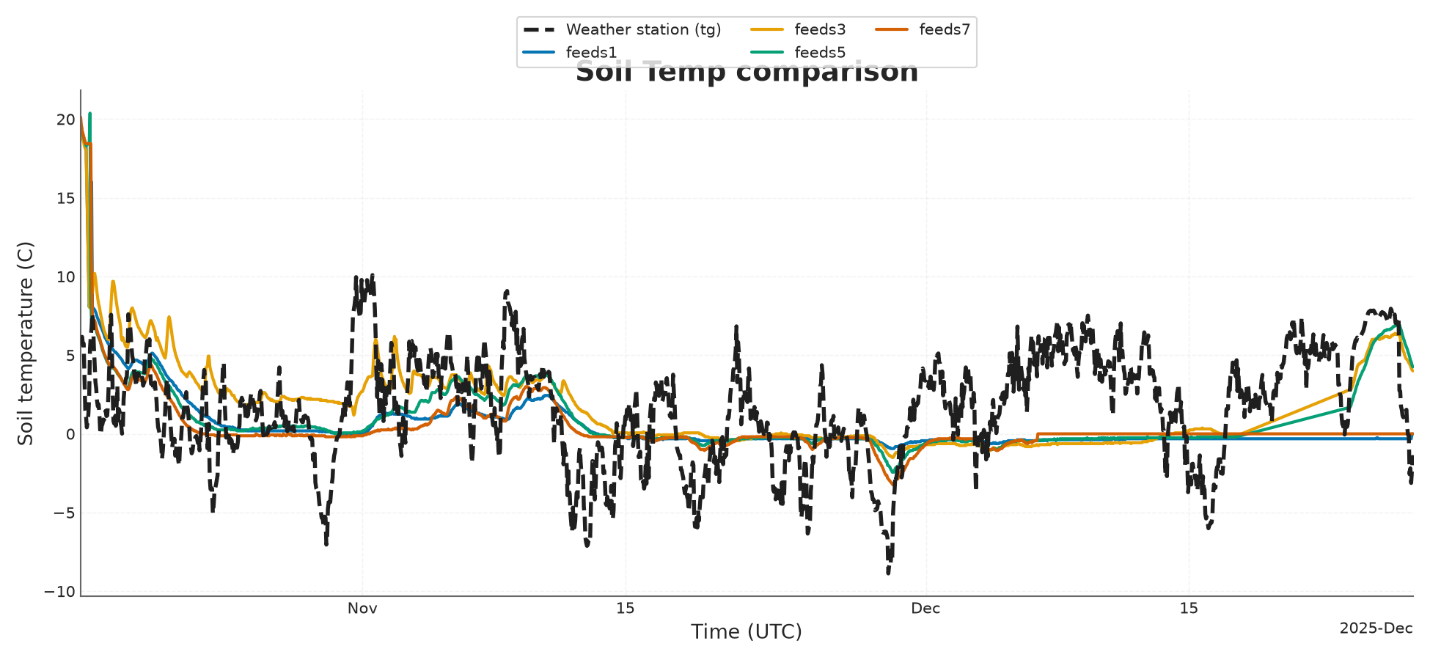
\includegraphics[width=\textwidth,height=3in,keepaspectratio]{figs/results-image9.png}
\caption{\draftchange{Comparison of soil temperature measurements from the deployed sensor nodes and ground-level data from the Sámsstaðir station (samst, 6222).}}
\label{fig:results-14}
\end{figure}

\draftchange{Unlike air temperature, soil temperature measurements from all four deployed nodes exhibited similar behavior regardless of installation configuration. The measured soil temperatures were significantly more stable than the air temperature recorded at station 6222, remaining close to the freezing point for much of the observation period. Rapid daily fluctuations in station 6222's air-temperature record were heavily damped by the thermal mass of the turf roof and surrounding soil.}

This behavior is expected since soil naturally buffers rapid temperature
changes. Even when air temperatures varied between approximately
\textbf{−8 °C and +10 °C}, soil temperatures remained close to \textbf{0
°C} with only gradual seasonal variation.

\draftchange{Station 6222 does \textbf{not} provide underground soil temperature measurements at the same depth as the deployed sensors. The comparison therefore used the station's \textbf{ground-level (surface) temperature} data as the closest available reference. Since the developed sensor nodes measured soil temperature at depths ranging from approximately \textbf{60 mm to 85 mm} below the turf surface (Figure~\ref{fig:results-deployment-map}), some difference between the two datasets was expected. Soil temperatures below the surface are naturally more thermally stable and less affected by rapid atmospheric temperature changes than temperatures measured at or near the ground surface.}

\draftchange{Consequently, the average absolute difference between the deployed sensor measurements and station 6222 data ranged from approximately \textbf{2.77 °C to 3.11 °C}. This is not a direct accuracy measurement, because the temperatures were measured at different locations and depths and under different environmental conditions. The Sámsstaðir comparison therefore does not independently validate the accuracy of the buried sensors.}

\draftchange{Overall, the measurements demonstrated stable soil-temperature trends during the deployment, consistent with the thermal buffering effect of the soil and turf. A reference sensor installed at the same location and depth as the deployed sensors would be required for a more direct comparison.}

\subsection{Individual Sensor
Performance}

\draftchange{The complete time-series measurements for Sensor Nodes 1, 3, 5, and 7 are presented in Figures~\ref{fig:results-15}, \ref{fig:results-16}, \ref{fig:results-8}, and \ref{fig:results-9}, respectively.}

\clearpage
\subparagraph{Sensor Node 1}

\draftchange{This node} maintained stable communication throughout most of the
deployment while continuously monitoring environmental conditions. Soil
moisture measurements remained relatively low with gradual increases
following wetter periods before decreasing as drainage occurred. Battery
voltage gradually decreased from approximately \textbf{4.1 V} to
\draftchange{\textbf{3.63 V}}, demonstrating efficient power consumption. \draftchange{The last valid ThingSpeak record from this node was received on 26 December 2025, an elapsed span of approximately 70.8 days from the first record. The final valid battery voltage was 3.63 V. The reason that subsequent valid measurements were no longer received is unknown.}

\begin{figure}[htbp]
\centering
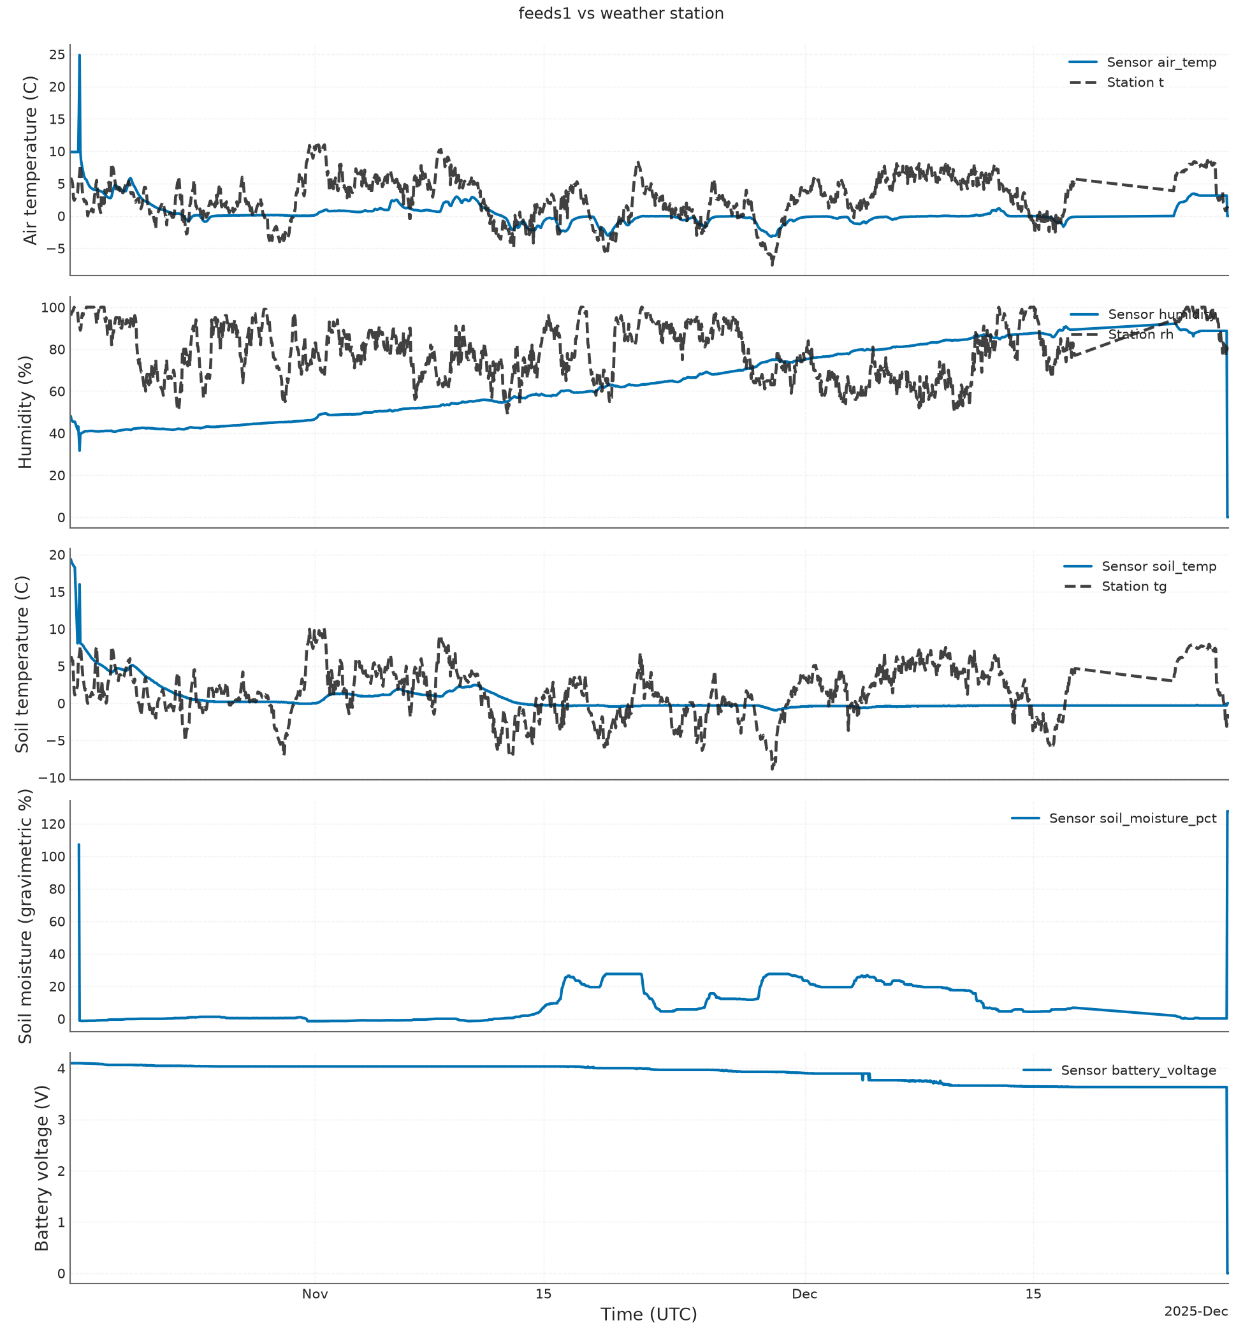
\includegraphics[width=5.63542in,height=6.06891in]{figs/results-image10.png}
\caption{Environmental measurements recorded by Sensor Node 1 throughout the deployment period.\draftchange{ Soil moisture is shown as raw ADC readings.}}
\label{fig:results-15}
\end{figure}

\clearpage
\subparagraph{Sensor Node 3}

\draftchange{Sensor Node 3 produced the longest valid ThingSpeak record, with a first-to-last valid reporting span of approximately 129.5 days, ending on 23 February 2026. The final valid entry reported a battery voltage of 3.49 V. This span includes the common interruption described in Section~\ref{sec:keldur-overall} and therefore does not represent uninterrupted uploads or a confirmed battery lifetime. The relative humidity readings from this node remained close to 100\% for an extended period near the end of its record and should be treated cautiously (Section~\ref{sec:keldur-humidity}).} \draftchange{Soil moisture increased during wetter conditions before gradually decreasing as the roof dried. Battery voltage showed a smooth and consistent discharge profile while the node was reporting.}

\begin{figure}[htbp]
\centering
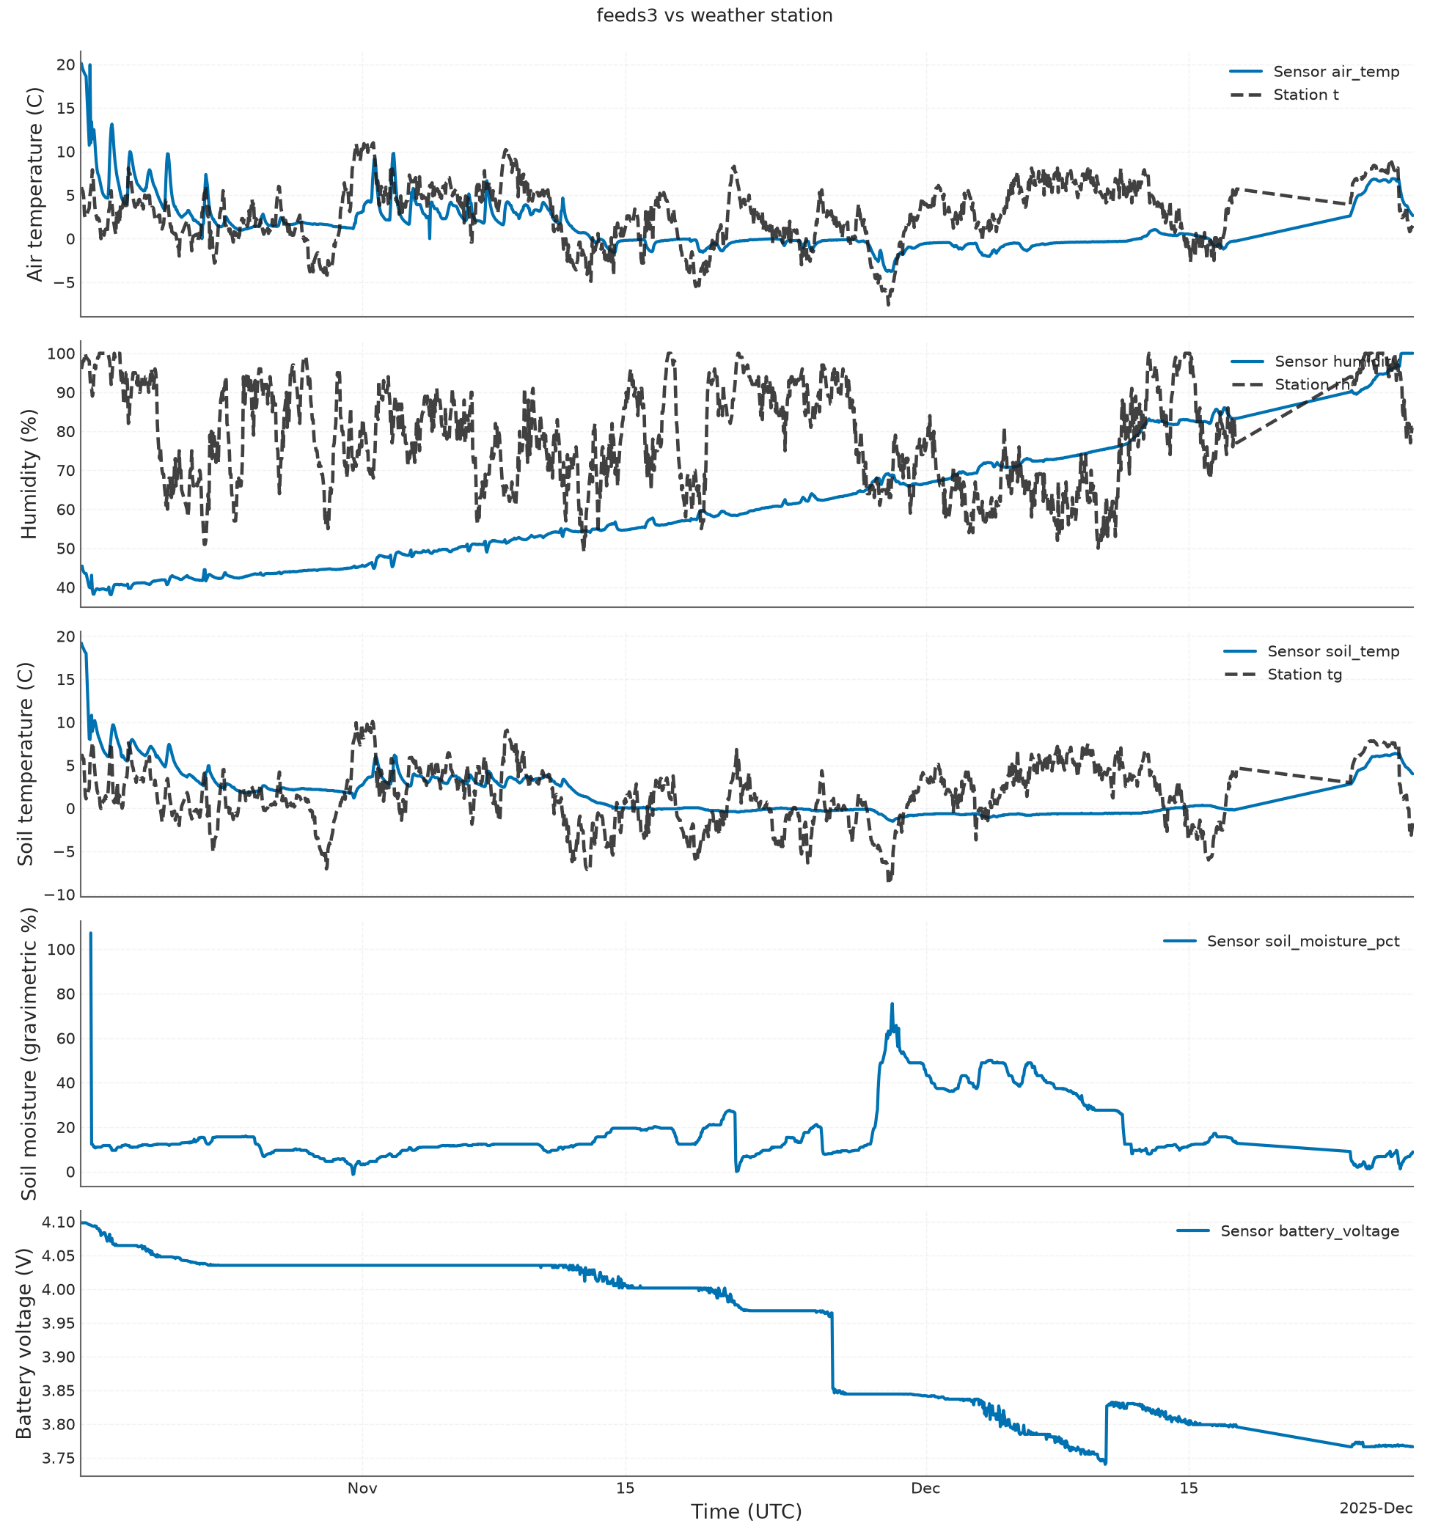
\includegraphics[width=\textwidth,height=7in,keepaspectratio]{figs/results-image11.png}
\caption{Environmental measurements recorded by Sensor Node 3 throughout the deployment period.\draftchange{ Soil moisture is shown as raw ADC readings.}}
\label{fig:results-16}
\end{figure}

\clearpage
\subparagraph{Sensor Node 5}

\draftchange{This node produced air temperature measurements that closely matched station 6222, consistent with its externally mounted atmospheric sensors. Its relative humidity readings are discussed in Section~\ref{sec:keldur-humidity}. Soil moisture remained consistently higher than the other deployed nodes, suggesting that its installation location retained more water within the turf roof. The reported battery voltage decreased gradually during the period for which valid measurements were received. The last valid ThingSpeak record was received on 2 January 2026, an elapsed span of approximately 77.5 days from the first record, with a final valid battery voltage of 3.78 V.}

\begin{figure}[htbp]
\centering
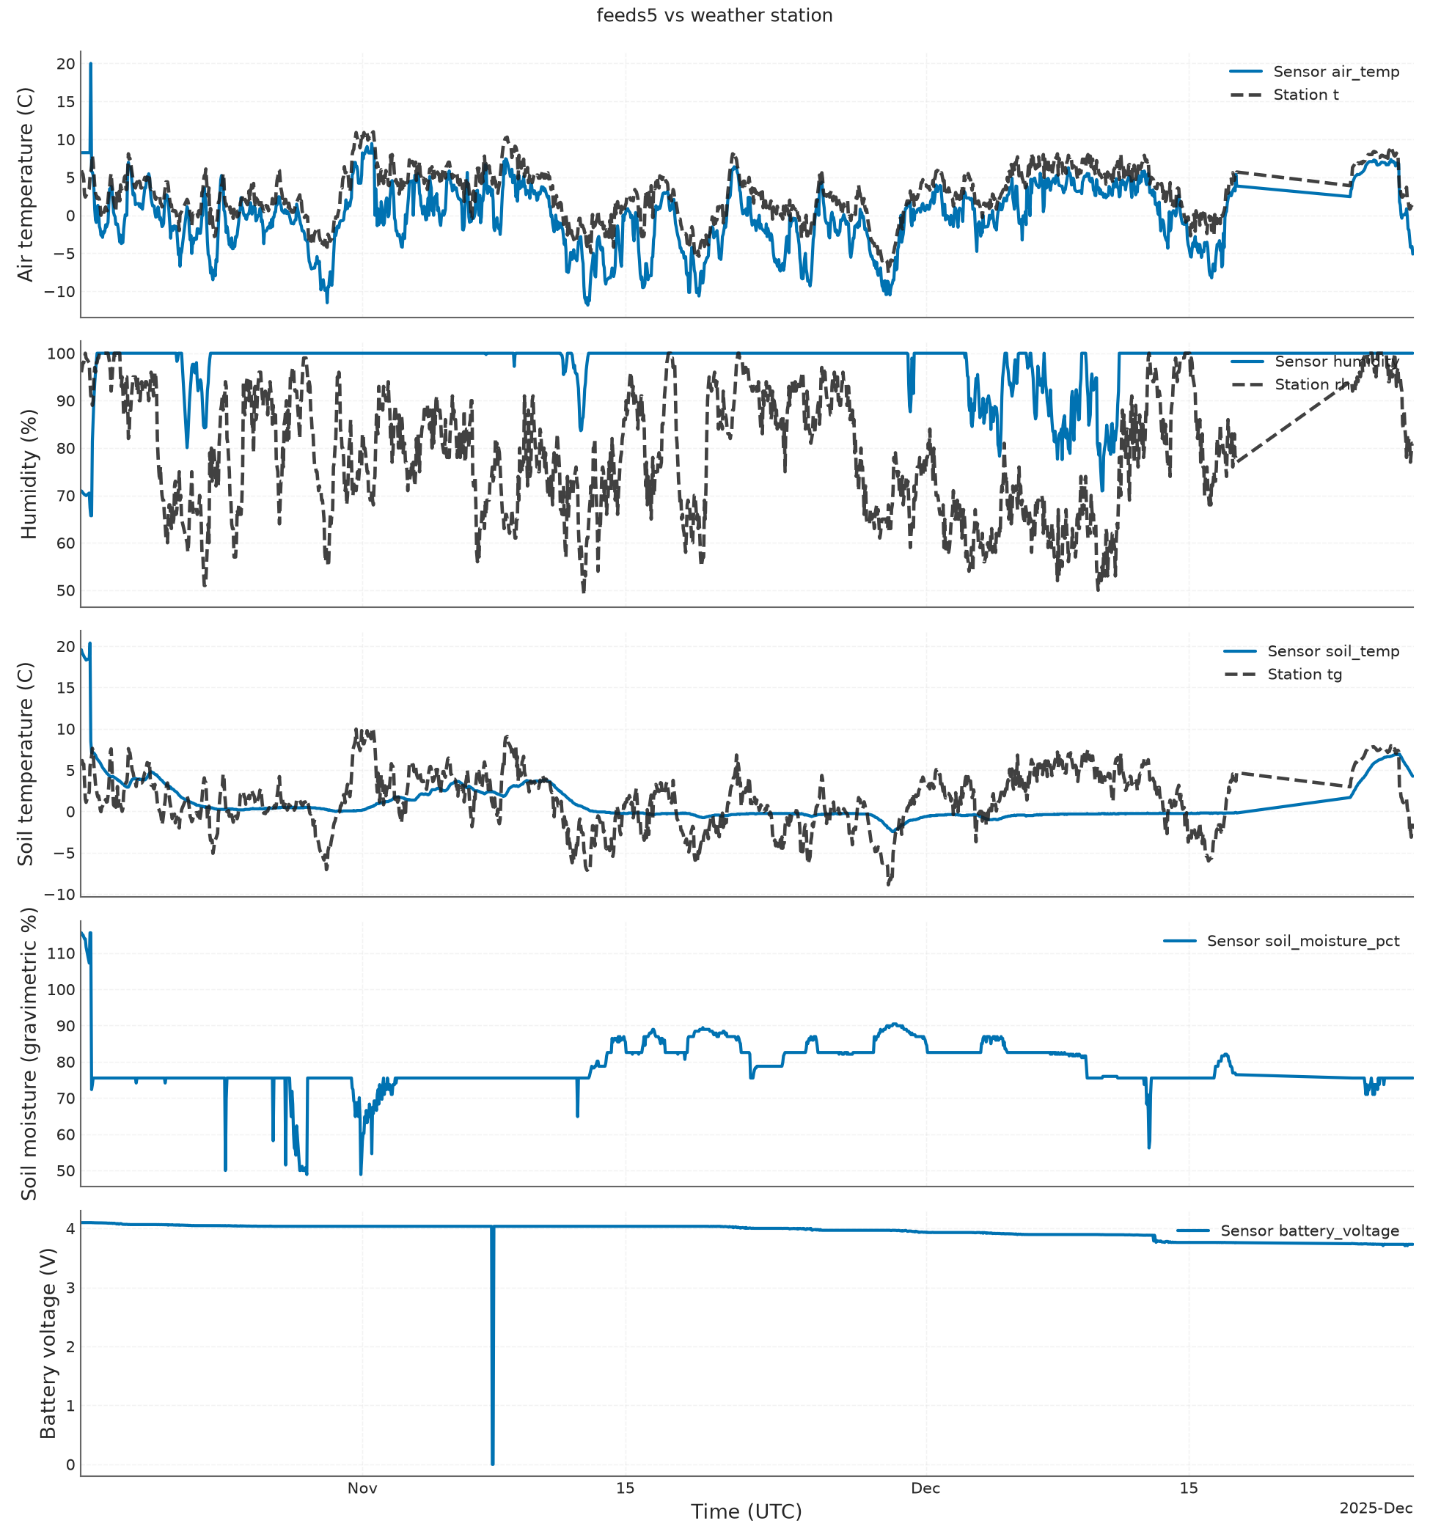
\includegraphics[width=\textwidth,height=7in,keepaspectratio]{figs/results-image12.png}
\caption{Environmental measurements recorded by Sensor Node 5 throughout the deployment period.\draftchange{ Soil moisture is shown as raw ADC readings.}}
\label{fig:results-8}
\end{figure}

\clearpage
\subparagraph{Sensor Node 7}

\draftchange{Sensor Node 7 provided valid measurements from 17 October 2025 through 6 December 2025, an elapsed span of approximately 50.9 days. The last valid ThingSpeak record reported a battery voltage of 3.93 V. The subsequent all-zero entries in the ThingSpeak feed are placeholders for missing measurements, not genuine zero-voltage or zero-humidity readings. The reason that this node stopped providing valid measurements is unknown.}

\begin{figure}[htbp]
\centering
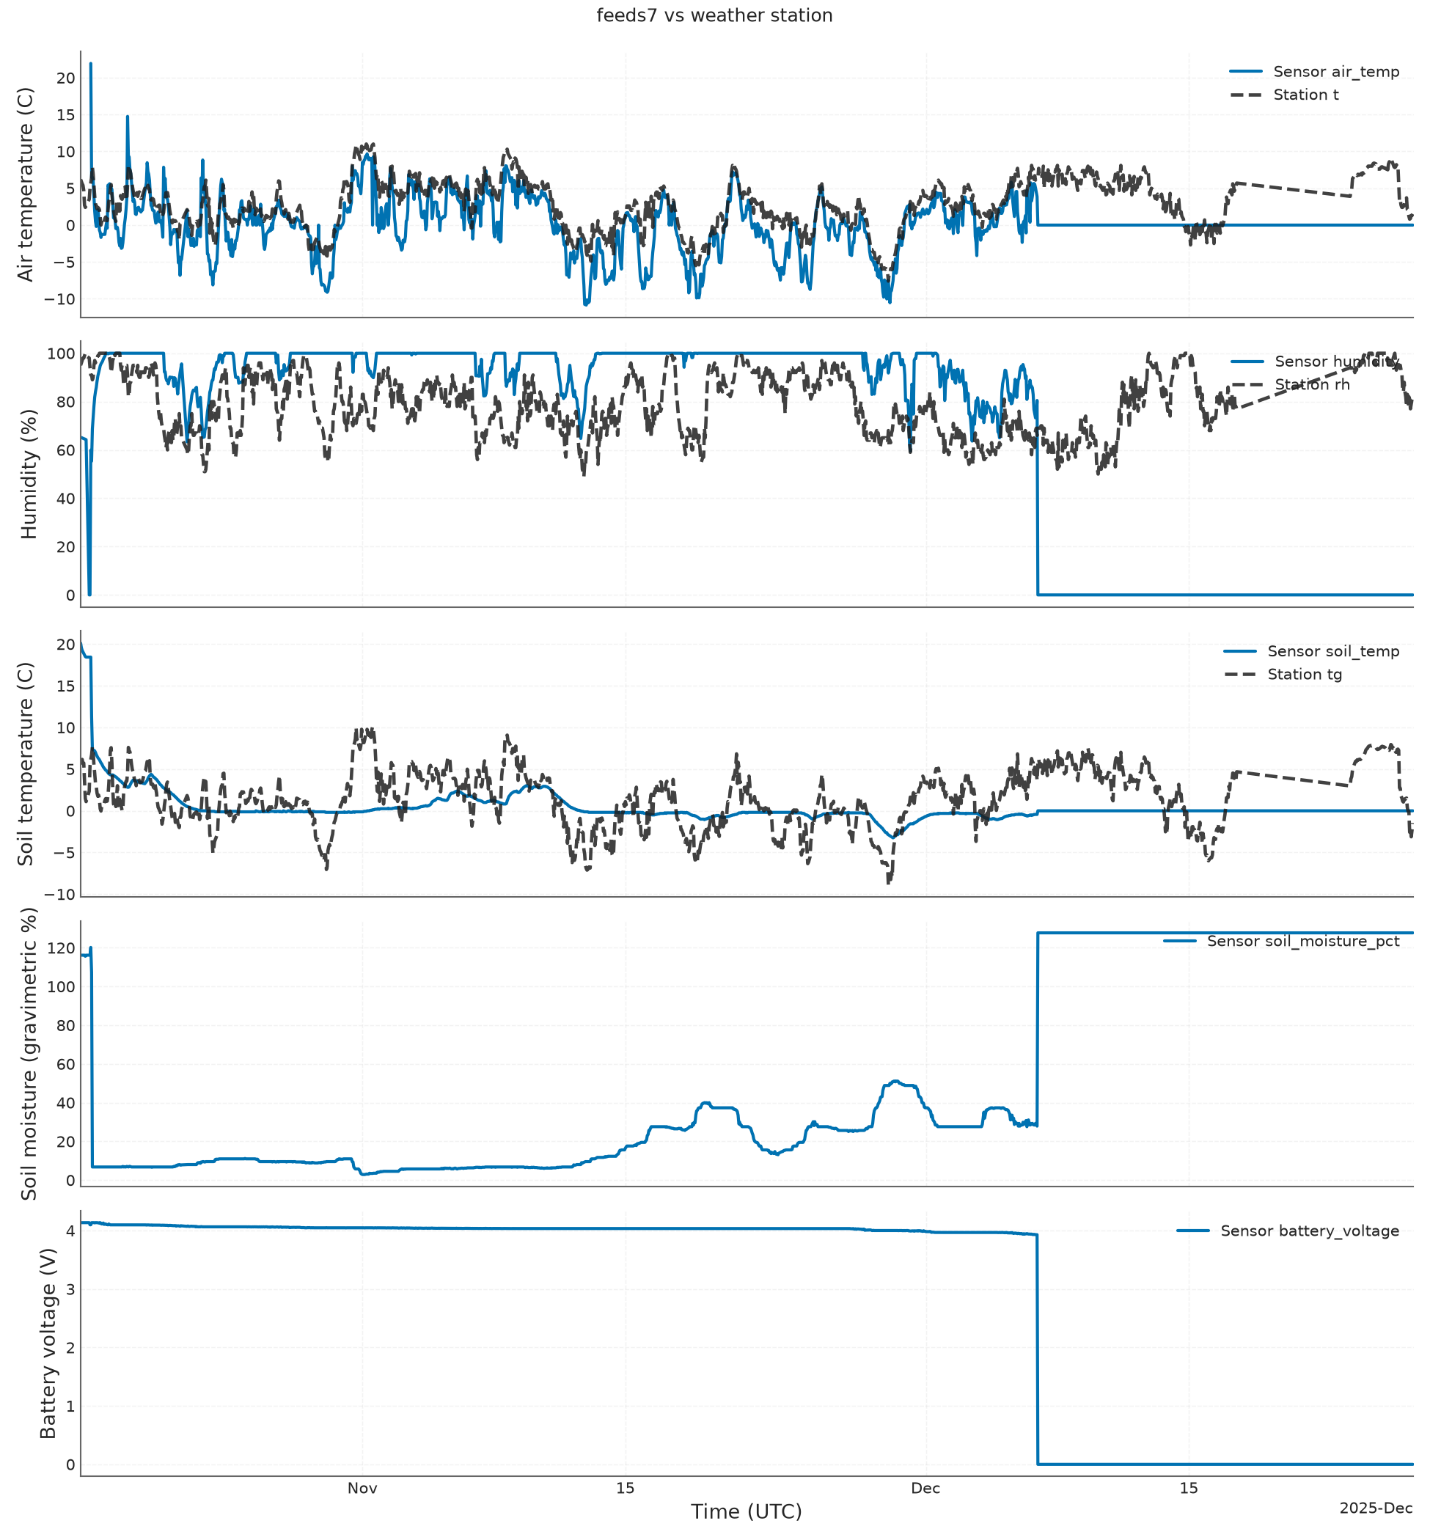
\includegraphics[width=\textwidth,height=7in,keepaspectratio]{figs/results-image13.png}
\caption{Environmental measurements recorded by Sensor Node 7 throughout the deployment period.\draftchange{ Soil moisture is shown as raw ADC readings.}}
\label{fig:results-9}
\end{figure}

\begin{table}[htbp]
\centering
\caption{\draftchange{Summary of valid ThingSpeak records and final reported battery voltages for the four Keldur sensor nodes.}}
\label{tab:keldur-record-span}
\begingroup
\color{purple}
\begin{tabular}{l l l c c}
\hline
Node & First record & Last record & Elapsed span & Final battery \\
\hline
1 & 17 Oct 2025 & 26 Dec 2025 & $\sim$70.8 days & 3.63 V \\
3 & 17 Oct 2025 & 23 Feb 2026 & $\sim$129.5 days & 3.49 V \\
5 & 17 Oct 2025 & 2 Jan 2026 & $\sim$77.5 days & 3.78 V \\
7 & 17 Oct 2025 & 6 Dec 2025 & $\sim$50.9 days & 3.93 V \\
\hline
\end{tabular}
\endgroup
\end{table}

\draftchange{The periods shown in Table~\ref{tab:keldur-record-span} represent the elapsed time between the first and last valid records received by ThingSpeak for each sensor node. They should not be interpreted as uninterrupted operating times or confirmed battery lifetimes, since missing records occurred during the deployment. The timestamps are based on the ThingSpeak \texttt{created\_at} field and therefore represent upload times rather than the sensor nodes' internal RTC measurement timestamps.}

\draftchange{The final valid battery voltages recorded for all four nodes remained above the configured 3.25 V cutoff. Since the sensor nodes were not retrieved at the end of the deployment, the reason each node stopped providing valid measurements could not be confirmed. Battery depletion should therefore not be presented as the cause.}

\draftchange{The ThingSpeak exports also contain all-zero entries after the last valid record of Sensor Nodes 1, 5, and 7. The base-station firmware clears its measurement arrays to zero at the start of each collection cycle, so when no valid new measurement is received from a node, these values can be uploaded as placeholders. These entries represent missing measurements rather than actual zero sensor readings. The soil-moisture values shown in the node plots are raw ADC readings from the capacitive sensors and are not converted to moisture percentages.}

\subsection{Overall System
Performance}\label{sec:keldur-overall}

\draftchange{The Keldur deployment demonstrated that the developed sensor nodes and base station could be installed beneath four separate turf roofs and used to collect environmental measurements under real outdoor conditions. The system recorded soil moisture, soil temperature, air temperature, relative humidity, and battery voltage, with measurements from the deployed nodes being delivered to ThingSpeak over different reporting periods.}

\draftchange{The reporting periods varied between nodes. Based on the first and last valid ThingSpeak records (Table~\ref{tab:keldur-record-span}), the elapsed spans ranged from approximately 50.9 days for Sensor Node 7 to 129.5 days for Sensor Node 3. These periods included missing records and should not be interpreted as uninterrupted operation or confirmed battery life. The last valid battery voltages were between 3.49 V and 3.93 V, all above the configured 3.25 V cutoff. Since the nodes were not retrieved, the reasons for the individual reporting endpoints remain unknown.}

\draftchange{A common interruption of approximately 145 hours was observed in the valid records from Sensor Nodes 1, 3, and 5, between 17 December and 23 December 2025. The available data do not identify the cause. Since these nodes experienced a similar interruption, it may have affected a shared part of the data collection or upload path. However, there are no retained base-station logs that would allow the interruption to be attributed to the LoRa communication, base station, internet connection, or another specific cause. Sensor Node 7 had already stopped providing valid measurements earlier, on 6 December 2025.}

\draftchange{The mesh communication algorithm was enabled on all four deployed sensor nodes. The firmware allowed nodes to receive, merge, and rebroadcast collected ledger data. However, no base-station packet logs were retained during the Keldur deployment. Consequently, it is not possible to determine whether particular measurements reached the base station directly or were forwarded through another sensor node. The deployment demonstrates that the implemented system collected and delivered data from four nodes, but it does not provide quantitative evidence of the individual multi-hop routes used.}

\draftchange{The separate range test conducted at Vellir demonstrated single-hop communication over an approximate 3 km radius. Mesh networking was not enabled during that range test, so its results should not be presented as a measured multi-hop range. An informal multi-hop test was also performed during firmware development (Section~\ref{sec:informal-multihop}), in which spaced sensor nodes relayed data until it reached the base station. This test was observed through debugging output, but no detailed logs, distances, packet counts, or route records were retained. It therefore provides qualitative evidence of the relay functionality rather than a reproducible performance measurement.}

\draftchange{Local SD-card backup was tested successfully during earlier field testing (Section~\ref{sec:sd-backup-testing}), where locally stored measurements were used to fill gaps in the base-station dataset. However, the Keldur node SD cards have not been retrieved, so this backup test cannot be used to claim that the missing Keldur records were recovered.}

\draftchange{Overall, the Keldur deployment demonstrated the practical feasibility of installing and operating the developed monitoring system at a real turf-roof site. It also identified important limitations involving missing measurements, uncertain node reporting endpoints, sensor data quality, and the lack of packet-level logging. Further field testing with retained communication logs and retrieved local data would be required to quantify long-term reliability and multi-hop performance.}

\section{Soil Moisture Calibration
Results}

\draftchange{The calibration results compare three measurement methods:
the gravimetric reference method, the HOBO MX2307 data logger,
and the custom capacitive soil moisture sensor.}

\subsection{Gravimetric Reference
Data}

Soil moisture calibration was performed using controlled samples at 0\%,
10\%, 20\%, 30\%, and 40\% moisture content. The gravimetric method was
used as the reference by adding known volumes of water to a measured
mass of dry soil.

Calibration was limited to 40\% moisture, as the soil approached
saturation beyond this point. Additional water produced minimal
dielectric variation, reducing the sensitivity of capacitive
measurements. \draftchange{The laboratory setup is shown in Figure~\ref{fig:calibration-setup}.}

\begin{figure}[htbp]
\centering
\subfigure[Calibration setup with the soil sample, custom sensors, and reference instrument.]{%
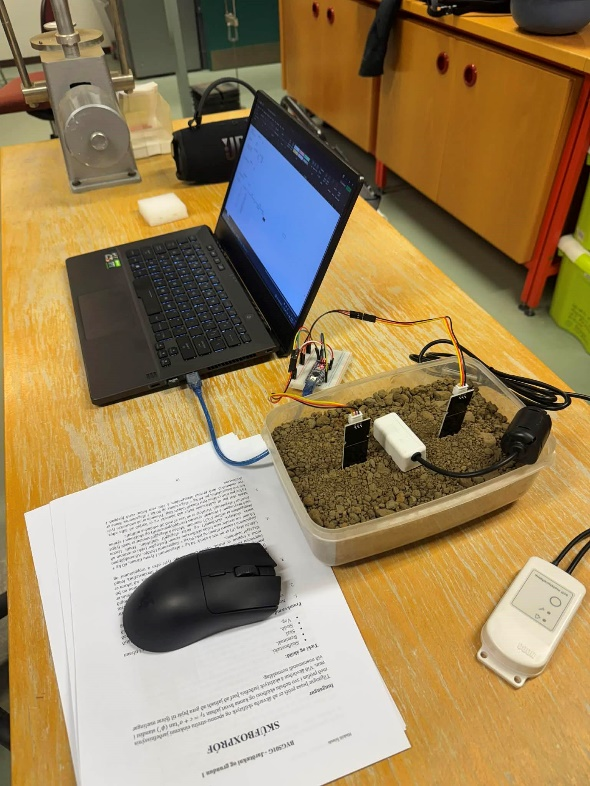
\includegraphics[width=2.67708in,height=3.56944in]{figs/results-image14.jpeg}}
\hfill
\subfigure[Custom sensors installed in the prepared soil sample.]{%
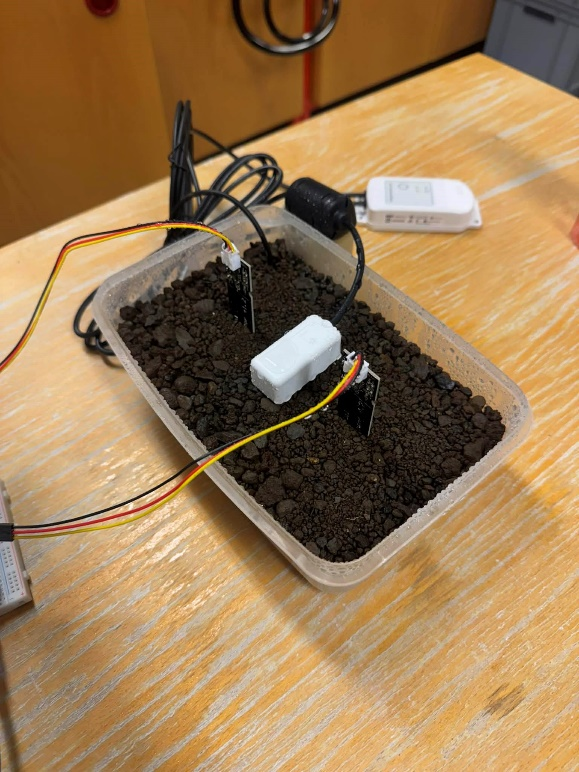
\includegraphics[width=2.67708in,height=3.56944in]{figs/results-image15.jpeg}}
\caption{Laboratory setup used for the soil moisture sensor calibration tests.}
\label{fig:calibration-setup}
\end{figure}

\clearpage
Two calibration tests were conducted.

\textbf{Test 1 (2069.5 g soil sample):}

\begin{longtable}[]{@{}
  >{\raggedright\arraybackslash}p{(\columnwidth - 8\tabcolsep) * \real{0.2254}}
  >{\raggedright\arraybackslash}p{(\columnwidth - 8\tabcolsep) * \real{0.2361}}
  >{\raggedright\arraybackslash}p{(\columnwidth - 8\tabcolsep) * \real{0.1758}}
  >{\raggedright\arraybackslash}p{(\columnwidth - 8\tabcolsep) * \real{0.1804}}
  >{\raggedright\arraybackslash}p{(\columnwidth - 8\tabcolsep) * \real{0.1822}}@{}}
\caption{Calibration Test 1 results for the 2069.5 g soil sample.}
\label{tab:calibration-test-1}\\
\toprule\noalign{}
\begin{minipage}[b]{\linewidth}\raggedright
\textbf{Soil Moisture (\%)}
\end{minipage} & \begin{minipage}[b]{\linewidth}\raggedright
\textbf{Water Added (mL)}
\end{minipage} & \begin{minipage}[b]{\linewidth}\raggedright
\textbf{VWC (m³/m³)}
\end{minipage} & \begin{minipage}[b]{\linewidth}\raggedright
\textbf{Raw Sensor 1}
\end{minipage} & \begin{minipage}[b]{\linewidth}\raggedright
\textbf{Raw Sensor 2}
\end{minipage} \\
\midrule\noalign{}
\endfirsthead
\endhead
\bottomrule\noalign{}
\endlastfoot
0 & 0 & 0 & 483.52 & 486.26 \\
10 & 206.95 & 0.15 & 314.17 & 324.55 \\
20 & 413.9 & 0.27 & 232.17 & 239.29 \\
30 & 620.85 & 0.33 & 223.26 & 216.67 \\
40 & 827.8 & 0.39 & 193.20 & 201.16 \\
\end{longtable}

The large sample size resulted in long saturation times and difficult
handling.

\textbf{Test 2 (400 g soil sample):}

\begin{longtable}[]{@{}
  >{\raggedright\arraybackslash}p{(\columnwidth - 6\tabcolsep) * \real{0.2750}}
  >{\raggedright\arraybackslash}p{(\columnwidth - 6\tabcolsep) * \real{0.2881}}
  >{\raggedright\arraybackslash}p{(\columnwidth - 6\tabcolsep) * \real{0.2145}}
  >{\raggedright\arraybackslash}p{(\columnwidth - 6\tabcolsep) * \real{0.2224}}@{}}
\caption{Calibration Test 2 results for the 400 g soil sample.}
\label{tab:calibration-test-2}\\
\toprule\noalign{}
\begin{minipage}[b]{\linewidth}\raggedright
\textbf{Soil Moisture (\%)}
\end{minipage} & \begin{minipage}[b]{\linewidth}\raggedright
\textbf{Water Added (mL)}
\end{minipage} & \begin{minipage}[b]{\linewidth}\raggedright
\textbf{VWC (m³/m³)}
\end{minipage} & \begin{minipage}[b]{\linewidth}\raggedright
\textbf{Raw Sensor 1}
\end{minipage} \\
\midrule\noalign{}
\endfirsthead
\endhead
\bottomrule\noalign{}
\endlastfoot
0 & 0 & 0.02 & 482.55 \\
10 & 40 & 0.21 & 260.36 \\
20 & 80 & 0.29 & 265.29 \\
30 & 120 & 0.34 & 220.68 \\
40 & 160 & 0.39 & 202.52 \\
\end{longtable}

The second test improved practicality while maintaining consistent
trends. In both tests, ADC values decreased as moisture increased,
confirming expected capacitive sensor behavior.

\subsection{HOBO Sensor and Dielectric
Reference}

A HOBO MX2307 (TEROS-10 probe) was used as a reference. It measures
dielectric permittivity and converts it to volumetric water content
(VWC) using:

\begin{equation}
\theta = 4.3 \times 10^{- 6}\varepsilon^{3} - 5.5 \times 10^{- 4}\varepsilon^{2} + 2.92 \times 10^{- 2}\varepsilon - 5.3 \times 10^{- 2}
\label{eq:dielectric-moisture-calibration}
\end{equation}

Measured VWC values were back-calculated to obtain dielectric
permittivity:

\begin{longtable}[]{@{}
  >{\raggedright\arraybackslash}p{(\columnwidth - 4\tabcolsep) * \real{0.2233}}
  >{\raggedright\arraybackslash}p{(\columnwidth - 4\tabcolsep) * \real{0.3442}}
  >{\raggedright\arraybackslash}p{(\columnwidth - 4\tabcolsep) * \real{0.4325}}@{}}
\caption{HOBO reference measurements and calculated dielectric permittivity.}
\label{tab:hobo-dielectric-reference}\\
\toprule\noalign{}
\begin{minipage}[b]{\linewidth}\raggedright
\textbf{Moisture (\%)}
\end{minipage} & \begin{minipage}[b]{\linewidth}\raggedright
\textbf{HOBO VWC (m³/m³)}
\end{minipage} & \begin{minipage}[b]{\linewidth}\raggedright
\textbf{Dielectric Permittivity (ε)}
\end{minipage} \\
\midrule\noalign{}
\endfirsthead
\endhead
\bottomrule\noalign{}
\endlastfoot
0 & 0.01 & 2.251 \\
10 & 0.18 & 9.578 \\
20 & 0.28 & 15.273 \\
30 & 0.335 & 19.175 \\
40 & 0.39 & 23.957 \\
\end{longtable}

Dielectric permittivity increased with moisture due to the high
dielectric constant of water.

\subsection{Polynomial Calibration
Model}

Due to the nonlinear relationship between ADC output and soil moisture,
a second-order polynomial regression was applied:

\begin{equation}
\text{Soil~Moisture~(\%)} = 0.0006877(\text{ADC})^{2} - 0.5961(\text{ADC}) + 127.70
\label{eq:adc-soil-moisture-calibration}
\end{equation}

\draftchange{The second-order polynomial was fitted using the arithmetic mean of the two capacitive sensor readings from Test 1 at each gravimetric moisture level. The resulting coefficients are presented in Equation~\ref{eq:adc-soil-moisture-calibration}. Table~\ref{tab:averaged-calibration-data} separately summarizes the average of all three capacitive sensor readings collected across both calibration tests. The two datasets should not be confused: the polynomial coefficients correspond to the Test 1 averages shown in Table~\ref{tab:final-calibration-results}, rather than the combined averages in Table~\ref{tab:averaged-calibration-data}.}

\begin{longtable}[]{@{}
  >{\raggedright\arraybackslash}p{(\columnwidth - 4\tabcolsep) * \real{0.3592}}
  >{\raggedright\arraybackslash}p{(\columnwidth - 4\tabcolsep) * \real{0.2606}}
  >{\raggedright\arraybackslash}p{(\columnwidth - 4\tabcolsep) * \real{0.3802}}@{}}
\caption{\draftchange{Overall average calibration data from both tests (all three capacitive sensor readings); these are not the input data used for the polynomial in Equation~\ref{eq:adc-soil-moisture-calibration}.}}
\label{tab:averaged-calibration-data}\\
\toprule\noalign{}
\begin{minipage}[b]{\linewidth}\raggedright
\textbf{Moisture (\%)}
\end{minipage} & \begin{minipage}[b]{\linewidth}\raggedright
\textbf{Avg VWC}
\end{minipage} & \begin{minipage}[b]{\linewidth}\raggedright
\textbf{Raw Avg ADC}
\end{minipage} \\
\midrule\noalign{}
\endfirsthead
\endhead
\bottomrule\noalign{}
\endlastfoot
0 & 0.01 & 484.11 \\
10 & 0.18 & 299.69 \\
20 & 0.28 & 245.58 \\
30 & 0.335 & 220.20 \\
40 & 0.39 & 198.96 \\
\end{longtable}

\clearpage
\subsection{Final Calibration Results and
Discussion}

\begin{longtable}[]{@{}
  >{\raggedright\arraybackslash}p{(\columnwidth - 8\tabcolsep) * \real{0.2534}}
  >{\raggedright\arraybackslash}p{(\columnwidth - 8\tabcolsep) * \real{0.1114}}
  >{\raggedright\arraybackslash}p{(\columnwidth - 8\tabcolsep) * \real{0.1921}}
  >{\raggedright\arraybackslash}p{(\columnwidth - 8\tabcolsep) * \real{0.2096}}
  >{\raggedright\arraybackslash}p{(\columnwidth - 8\tabcolsep) * \real{0.2336}}@{}}
\caption{\draftchange{Comparison of gravimetric moisture, Test 1 mean ADC, HOBO, dielectric, and polynomial output values.}}
\label{tab:final-calibration-results}\\
\toprule\noalign{}
\begin{minipage}[b]{\linewidth}\raggedright
\textbf{Gravimetric (\%)}
\end{minipage} & \begin{minipage}[b]{\linewidth}\raggedright
\textbf{\draftchange{Test 1 Mean ADC}}
\end{minipage} & \begin{minipage}[b]{\linewidth}\raggedright
\textbf{HOBO VWC}
\end{minipage} & \begin{minipage}[b]{\linewidth}\raggedright
\textbf{Dielectric (ε)}
\end{minipage} & \begin{minipage}[b]{\linewidth}\raggedright
\textbf{\draftchange{Polynomial Output (\%)}}
\end{minipage} \\
\midrule\noalign{}
\endfirsthead
\endhead
\bottomrule\noalign{}
\endlastfoot
0 & 484.89 & 0.01 & 2.251 & \draftchange{0.35} \\
10 & 319.36 & 0.18 & 9.578 & \draftchange{7.47} \\
20 & 235.73 & 0.28 & 15.273 & \draftchange{25.40} \\
30 & \draftchange{219.97} & 0.335 & 19.175 & \draftchange{29.85} \\
40 & 197.18 & 0.39 & 23.957 & \draftchange{36.90} \\
\end{longtable}

\draftchange{The polynomial model produced an RMSE of approximately 3.01 percentage points when its calculated moisture values were compared with the gravimetric moisture targets at the five calibration levels. This value represents the fit error on the same calibration data used to derive the polynomial. It is therefore an in-sample calibration error rather than an independent validation result.}

\draftchange{For comparison, converting the HOBO VWC values to percentages and comparing them with the polynomial outputs gives an RMSE of approximately 5.21 percentage points over the same five calibration levels. This comparison provides an indication of the difference between the two measurement methods, but it should not be described as independent validation because the readings were collected during the same calibration procedure.}

\draftchange{The calibration was conducted using a separate Icelandic soil sample rather than soil collected from the Keldur deployment locations. Although the same capacitive sensor model and supply voltage were used, the soil composition and characteristics may differ. As a result, the calibration relationship cannot automatically be assumed to apply to all Keldur soil conditions.}

\draftchange{The Keldur ThingSpeak data further show that a substantial portion of the raw ADC readings falls outside the ADC range used to fit the polynomial, approximately 197.18--484.89. Using records with a non-zero battery-voltage field and excluding the all-zero placeholder entries, the median raw ADC values were approximately 527 for Node 1, 575 for Node 3, 768 for Node 5, and 568 for Node 7. Only approximately 31.1\% of Node 1 readings and 0.8\% of Node 3 readings fell within the calibration range. No readings from Nodes 5 and 7 fell within that range.}

\draftchange{These results mean that applying the polynomial to the full Keldur datasets would require extrapolation for most measurements. Such extrapolation would not be reliable. Therefore, the Keldur soil-moisture plots should remain in raw ADC units rather than being converted into volumetric water content or calibrated moisture percentages using this polynomial.}

\draftchange{The calibration demonstrates that the capacitive sensor has a nonlinear response to controlled changes in soil moisture over the tested 0--40\% range. However, further calibration using soil collected from the actual turf-roof locations, together with independent reference measurements, is required before quantitative soil-moisture values can be confidently reported for the Keldur deployment.}

\section{Cloud Upload Performance
(ThingSpeak)}

\draftchange{The cloud upload functionality was evaluated using the ThingSpeak IoT
platform. Sensor data from the base station---including soil moisture,
temperature, humidity, battery voltage, and timestamps---was transmitted
via Wi-Fi using HTTP GET requests. During testing, the uploaded sensor
data was successfully received by the ThingSpeak server, with the
requests consistently returning an HTTP response code of \emph{200 OK}.
The average upload time was approximately 1--2 seconds, depending on
network conditions.}

\draftchange{The integration made the collected sensor measurements available through ThingSpeak for remote access, visualization, and further analysis. The observed upload time was suitable for the periodic data-transfer requirements of the monitoring system.}

\draftchange{These results describe the controlled cloud-upload tests. They confirm that the upload process worked during the recorded tests, but they do not establish uninterrupted cloud availability or upload success throughout the Keldur field deployment.}
